\chapter{Results and Analysis}
\section{Signal Characteristics}\label{sec:sigChar}
In order to understand the nature of the problem there was requirment for pre-analysis of data. The primary dataset used is 2 seconds of electric field recordings, from a particular instance of exceedingly high lightning activity. This raw data was recorded with a sampling frequency $f_s = 1\si{\mega\hertz}$. These are broadband recordings, the time series is shown by Figure \ref{fig:realData} and the frequency spectrum of the recording is shown by the Figure \ref{fig:realFFT} shows that they cover the band of 0-300\si{\kilo\hertz}. The large spike at 198kHz is Radio 4's long wave service, this is an AM transmission hence it needs to have a very large amplitude to avoid background interference. Unlike the VLF signals we are interested in which are phase/frequency modulated, therefore the transmitted power lower.


\begin{figure}[h!]
    \begin{subfigure}[b]{0.5\textwidth}
        \centering
        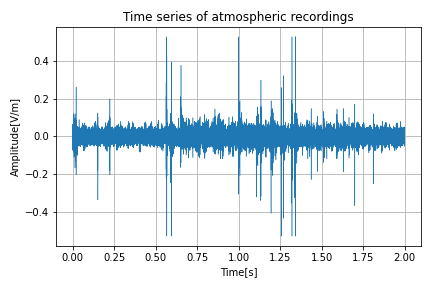
\includegraphics[width = \textwidth]{figs/sig_character/timeseries.png}
        \caption{Time Series}
        \label{fig:realData}
    \end{subfigure}
    \begin{subfigure}[b]{0.5\textwidth}
    `   \centering
        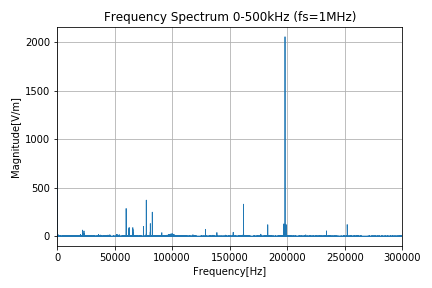
\includegraphics[width = \textwidth]{figs/sig_character/fft_data.png}
        \caption{FFT}
        \label{fig:realFFT}
    \end{subfigure}
    \caption{Unfiltered Real Data}
\end{figure}



Figure \ref{fig:vlfspect} is a spectrogram showing the band of interest to this problem and effectively represents the problem space. It can be seen in this plot that the vertical lines represent active transmitters of which there are five. The horizontal lines represent interference events. Figure \ref{fig:transSpect} shows the more localised contained the centre frequencies of the transmitters visible. This clearly illustrates the impulsive nature of noise, in this plot there are 4 visible impulses, the cause of which is the electromagnetic radiation produced by a lightning event. 

\begin{figure}[h!]
        \centering
        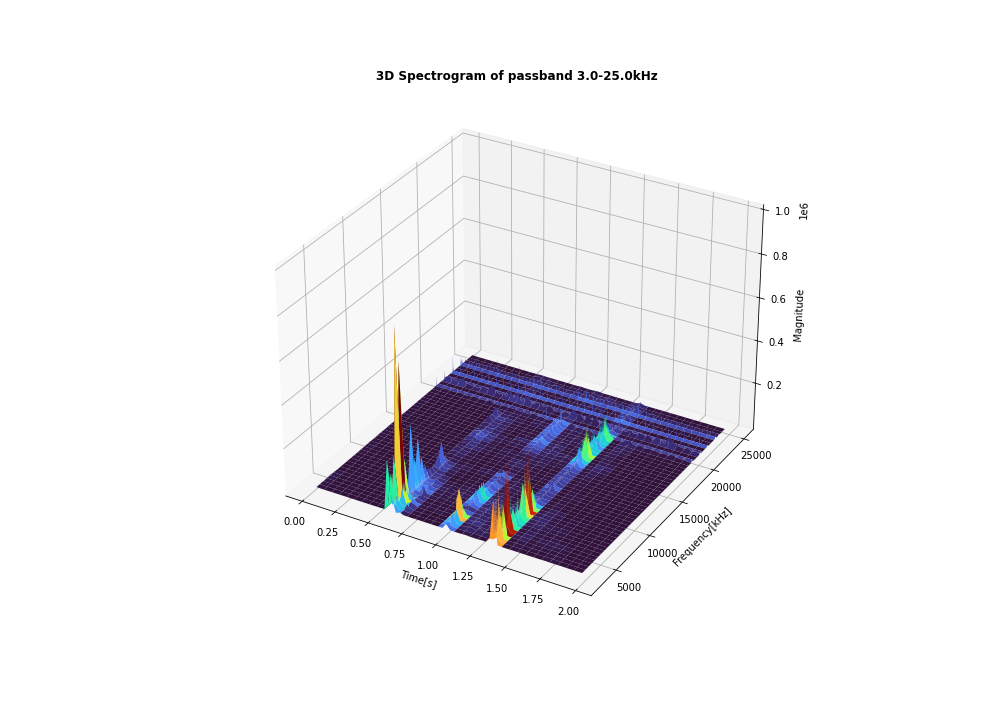
\includegraphics[width = \textwidth]{figs/sig_character/vlfspectrogram.png}
        \caption{3D spectrogram covering VLF band}
        \label{fig:vlfspect}
\end{figure}
\begin{figure}[h!]
        \centering
        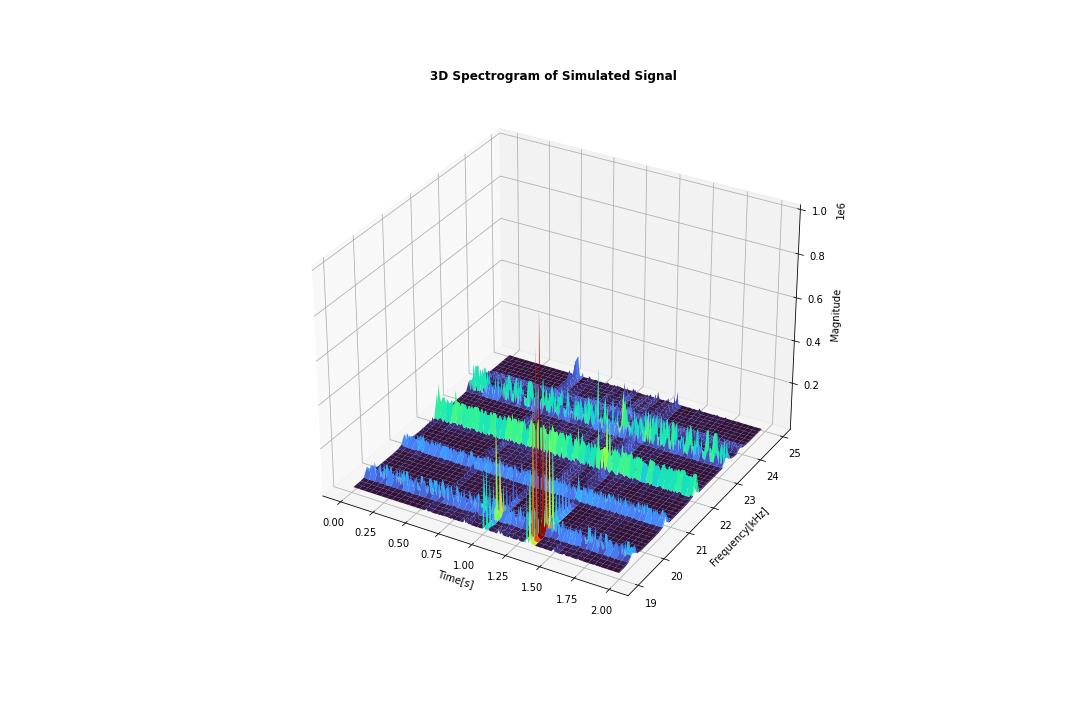
\includegraphics[width = \textwidth]{figs/sig_character/transmitters_spectrogram.png}
        \caption{Band containing active transmitters}
        \label{fig:transSpect}
\end{figure}

Figure \ref{fig:absAmplitude} shows the absolute amplitude of the five active transmitters that are in the recorded dataset. Additionally as described in section \ref{sec:investigations} the plots also show the limits used for noise bounding in order to estimate the noise signal for this example. $k=1.5$ has been used in order to set this limit. These properties are then used to calculate the noise signal and then in turn estimate to the Signal to Noise ratio. This estimate is calculated and shown by table \ref{tab:snr1}. By referring back to figure \ref{fig:transSpect} in addition to the amplitude plots, the spikier the plots are can justify the inference that there is much more interference present in the signal. 

\begin{figure}[h!]
    \centering
    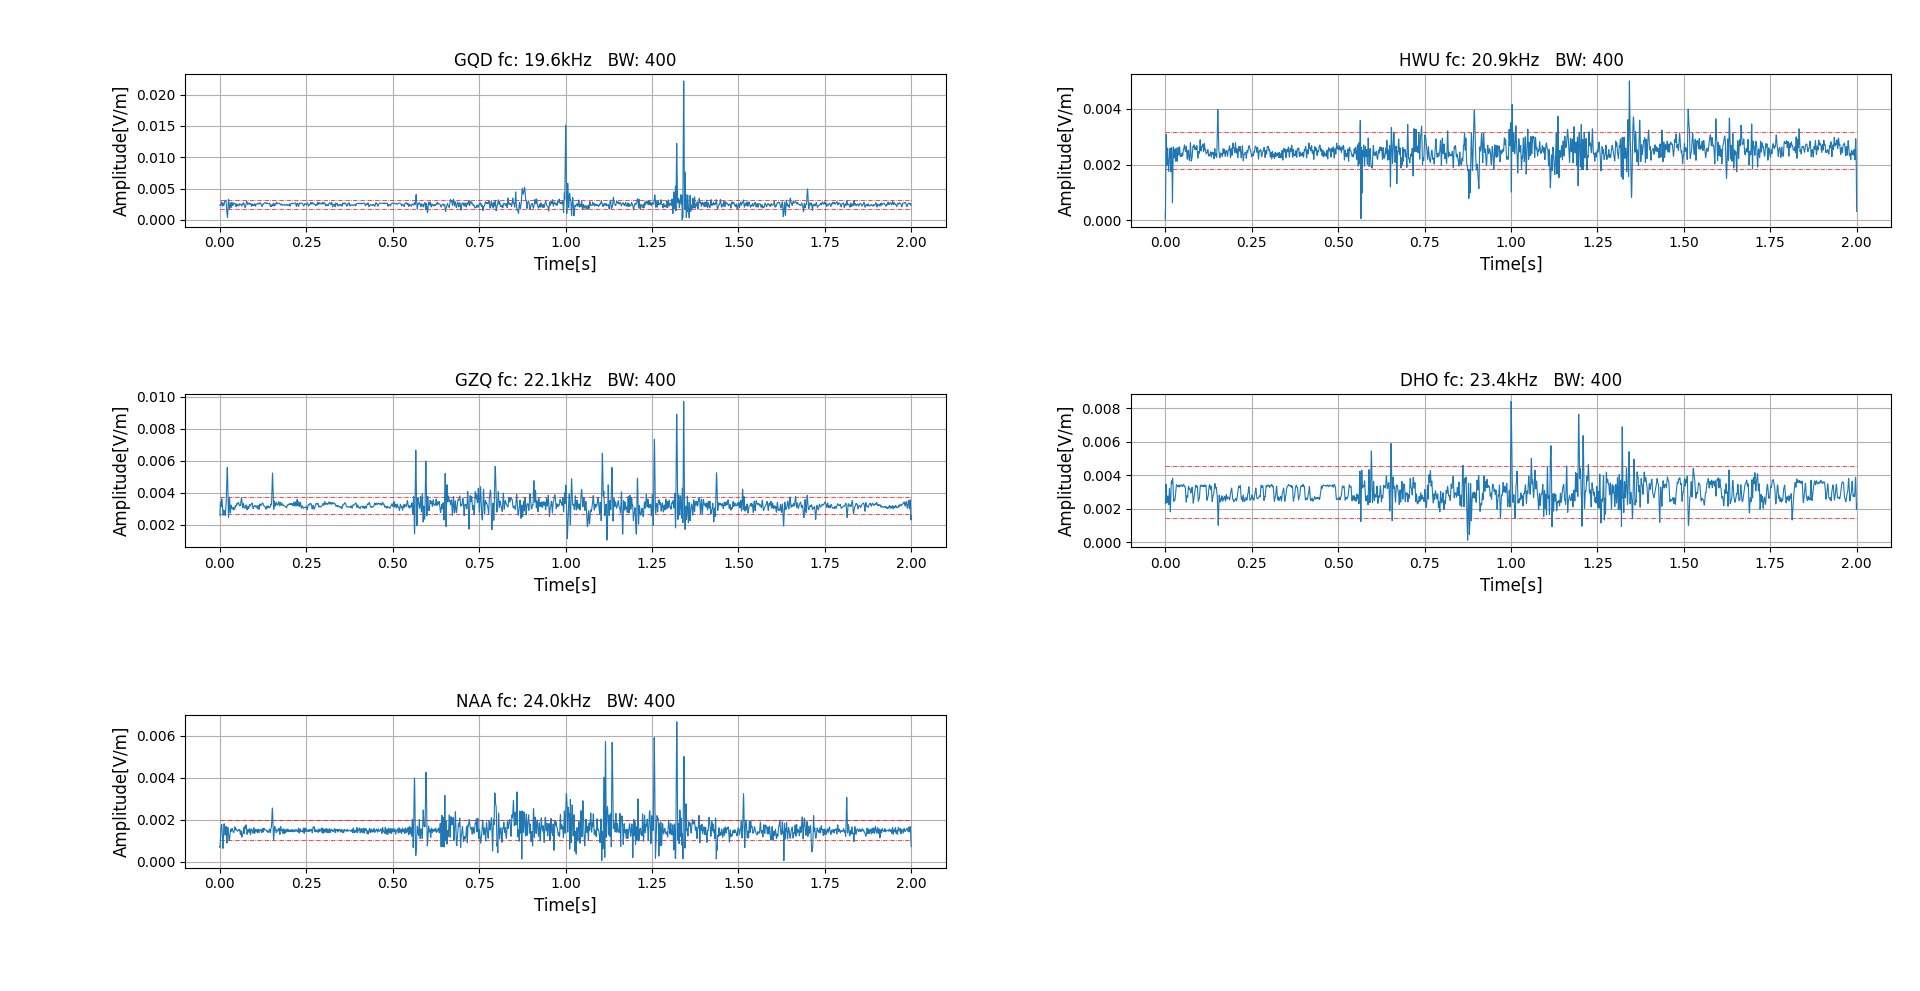
\includegraphics[width = \textwidth]{figs/sig_character/abs_amplitude.png}
    \caption{\centering Absolute Amplitude of Complex Trace of VLF Transmitters, shown with upper and lower limits for noise bounding.}
    \label{fig:absAmplitude}
\end{figure}

\begin{table}[h!]
\centering
    \begin{tabular}{l|l|l}
    Callsign & SNR [dB] & Centre Frequency $f_c$ [kHz] \\
    \hline
    GQD & 12.5 & 19.6 \\
    HWU & 25.5 & 20.9 \\
    GZQ & 16.8 & 22.1 \\
    DHO38 & 28.7 & 23.4 \\
    NAA & 9.9 & 24
    \end{tabular}
\caption{Estimated Signal to Noise ratio of VLF transmitters}
\label{tab:snr1}
\end{table}

Figure \ref{fig:gqd3d} shows the complex sinusoid received for the transmitter GQD. Although it is clearly corrupted by noise however the cylindrical shape represents the transmitter, where the signal deviates from this core 'cylinder', which ultimately represents the phasor of the transmitter, is as a result of atmospheric noise. 

\begin{figure}[h!]
    \centering
    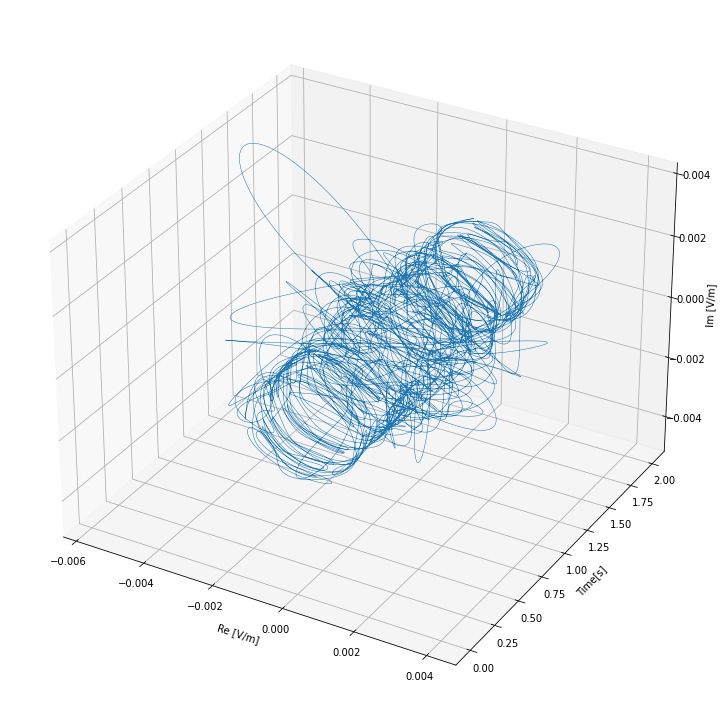
\includegraphics[width = \textwidth]{figs/sig_character/gqd3D.png}
    \caption{3D complext plot of transmitter GQD}
    \label{fig:gqd3d}
\end{figure}


Appendix X contains the figures related to the demodulated signals for each transmitter, as it is clear that MSK is used as the modulation technique illustrated by the constant frequency for each symbol, the gradient changes sign when the symbol changes. This represent a zero crossing in the first differential which corresponds to the instantaneous frequency. In all instances the passband of the orignal data has been $f_c \pm 400Hz$

\subsection{Noise Estimation}\label{sec:noiseEst}
As a key part of the investigation is to simulate the noise present in these VLF signals, it is important to accurately estimate the noise. As previously mentioned the aim is to this statistically by defining the noise as outliers within the data. Figure \ref{fig:noise estimate} shows the results of estimating the noise. By inspection it is clear that the noise is not consistent between all the transmitters, the most likely explanation of this is clipping in the data acquisition unit used to record the data. The restricts the maximum value to roughly 0.5 \si{\volt \per\metre}, as a result at the maximum values shown there is a local rectangular waveform. In the frequency domain this results in a sinc function. The result of this is that certain frequencies will result in a minimum and other in a maximum. This is clearly visible at 1.0\si{\second} where there is clearly a lightning event, because lightning events are broadband this event should be visible at all frequencies as is shown by some of the other less powerful spikes also present. That are the same across all the transmitters. The clipping instance at 1.0\si{\second} is shown by figure \ref{fig:clipping}, where the signal apparently takes on a rectangular characteristic which we know is not that case.

\begin{figure}[h!]
    \centering
    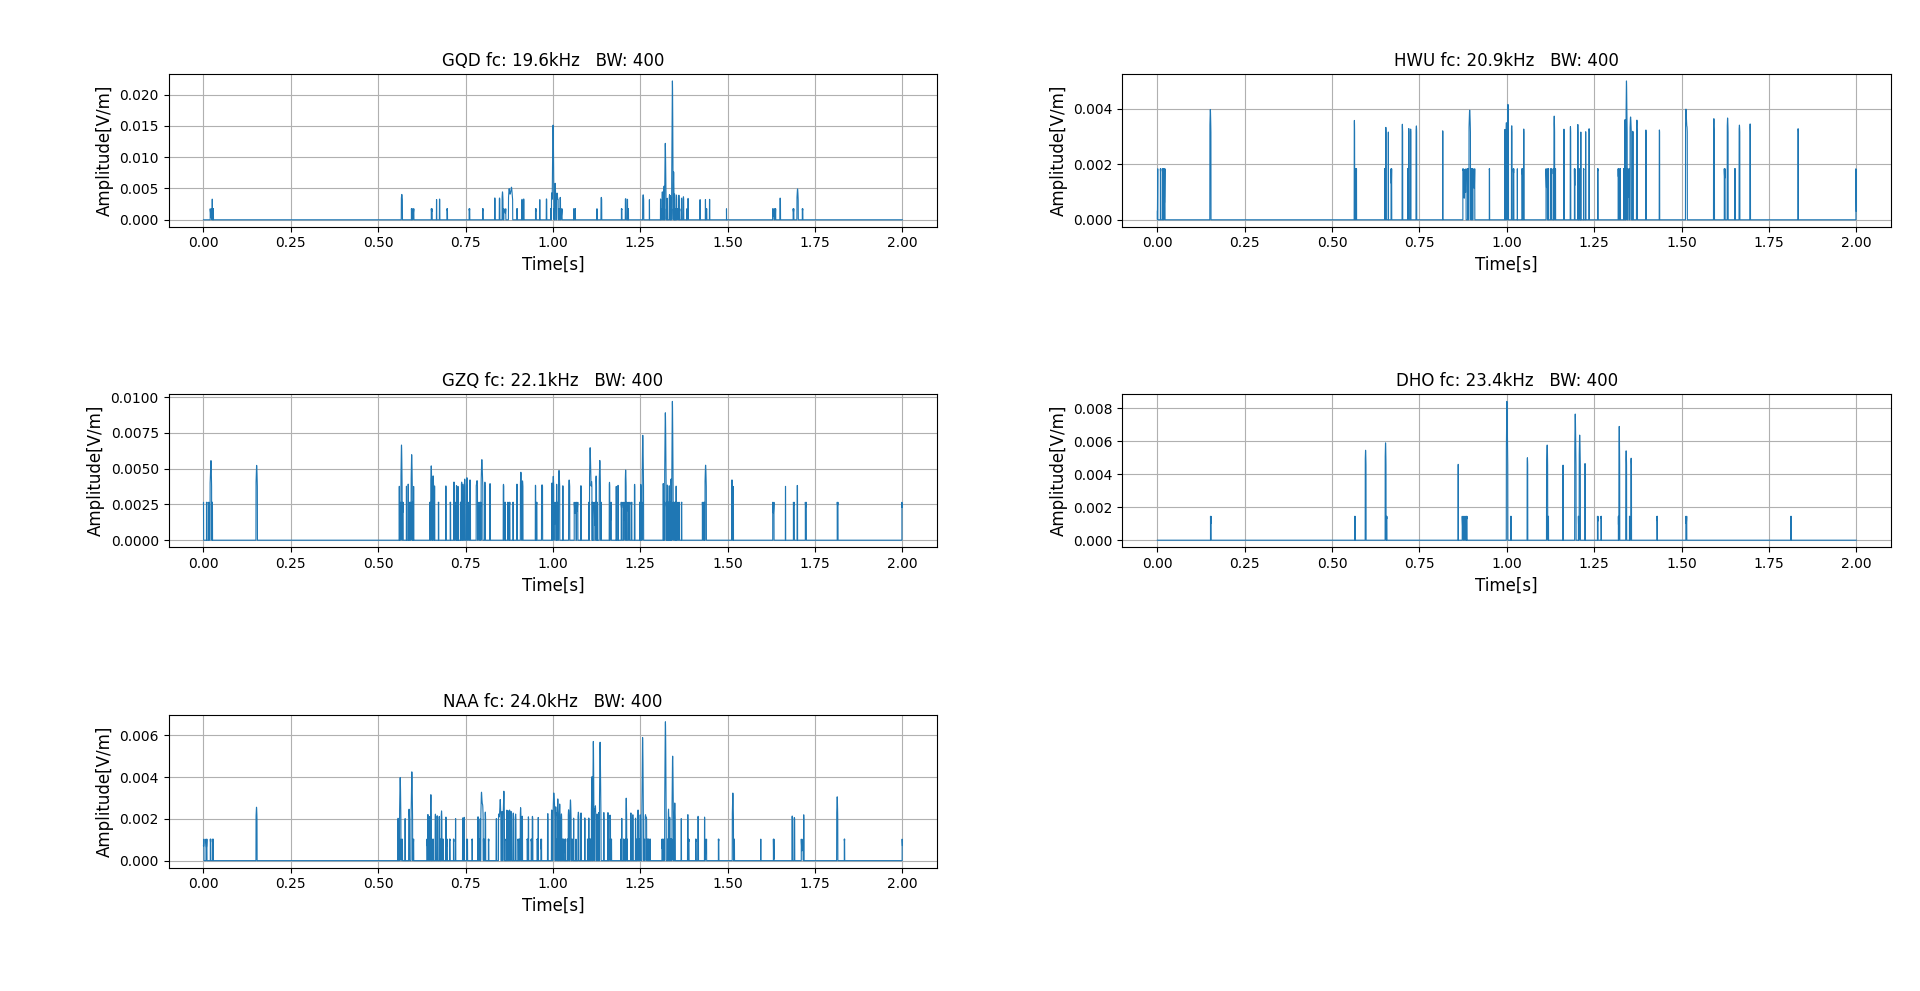
\includegraphics[width = \textwidth]{figs/sig_character/noiseEstimate.png}
    \caption{Estimated Noise Present within Recorded Data}
    \label{fig:noise estimate}
\end{figure}

\begin{figure}[h!]
    \centering
    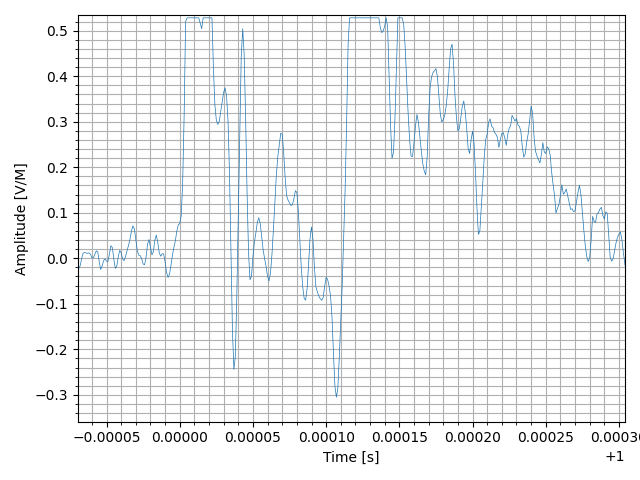
\includegraphics[width = \textwidth]{figs/sig_character/Clipping.png}
    \caption{Clipped Time Series Around 1.0s}
    \label{fig:clipping}
\end{figure}

The final thing to take from the figure \ref{fig:noise estimate} is that there are clearly two types of noise generated from different parts of the lightning event. These can be broadly characterised into two types of noise.
\begin{itemize}
    \item High Amplitude noise: This is a result of the return stroke, it is characterised by a large amplitude and has a duration in the order $10^{-6}\si{\second}$ 
    \item Intensive noise: This is characteristic of the continuous current, it generally has a lower amplitude but a longer duration to the order of $10^{-3}\si{\second}$

\end{itemize}

\pagebreak
\section{Simulation}
\subsection{Control Signal}
The development of a successful simulation was key in order to assess the problem as previously explained the MSK signal consists of an inphase and quadrature component, these are cosine and sine waves amplitude modulated with the pulse shaped baseband signal. This is shown by figure \ref{fig:carrier}, which shows these signals. The algorithm that converts the message signal to baseband is shown by listing \ref{lst:algorithm}
\begin{lstlisting}[language = python, captionpos=b, caption = Algorithm to create Correct signs for $a_{i}$ and $a_{q}$, label = lst:algorithm]
    for i in range(0,L-2):
        if i%2 == 0:
            if msgl[i] == msgl[i+1]:
                a = np.append(a, a[int(i/2)])
            elif msgl[i] != msgl[i+1]:
                a = np.append(a, a[int(i/2)]*-1)
        else:
            if msgl[i] == msgl[i+1]:
                b=np.append(b, b[int(np.floor(i/2))])
            elif msgl[i] != msgl[i+1]:
                b = np.append(b, b[int(np.floor(i/2))]*-1)
\end{lstlisting}
They are then combined in order to create the final signal that is suitable for transmission. The final complex waveform is shown by figure \ref{fig:3DBB}, where the symbol switch point can be seen. The baseband frequency is determined by the bitrate, which is $f_{1bb} = \frac{1}{T_b}$. This means that in theory there is potential for a bit change everytime there is an axis crossing, in reality this is eight points where the direction of the phasor can change either side of the axis, depending on which direction the phasor is moving depends on which one of these points it will switch. The rotating phasor is defined as $Z_{n}$ shown in equation \ref{eq:phasor}. These results have been simulated with a centre frequency of 22.1kHz and are to illustrate proof of concept for the simulation tools.

\begin{equation}
    Z_n = e^{2\pi f_{BW}t}
    \label{eq:phasor}
\end{equation}

\begin{figure}[h!]
    \centering
    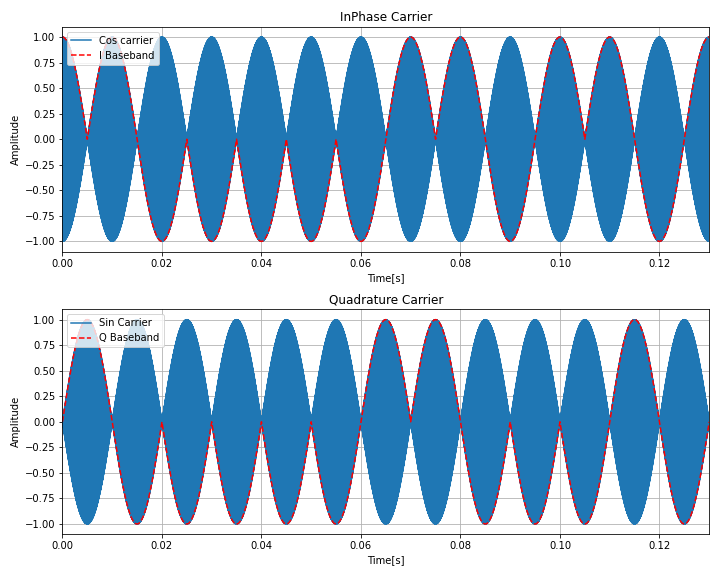
\includegraphics[width = \textwidth]{figs/sim/carrier.png}
    \caption{\centering Amplitude Modulated Cos and Sin carriers corresponding to Inphase and Quadrature elements}
    \label{fig:carrier}
\end{figure}
\begin{figure}[h!]
    \centering
    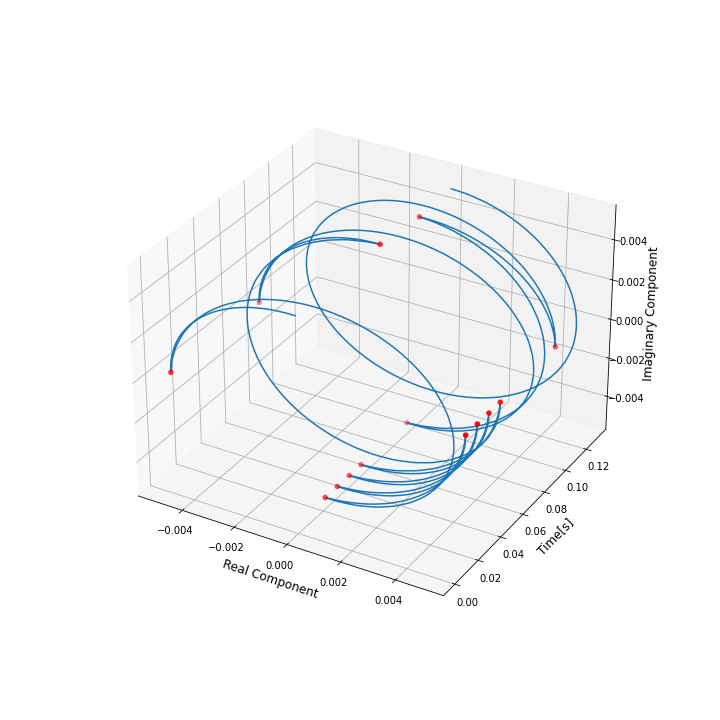
\includegraphics[height = \textwidth]{figs/sim/3dbaseband.png}
    \caption{3D Baseband Plot $fc = 22.1\si{\kilo\hertz}$. \small{Red Markers highlight symbol changes}}
    \label{fig:3DBB}
\end{figure}

Figure \ref{fig:simDemod} illustrates the output the desired output signal at the receiver, it is important to note that this is in an ideal signal so therefore it produces an ideal output. The oscillations in each bit are a transient response to the sharp change in frequency as a result of a bit change. 

\begin{figure}[h!]
    \centering
    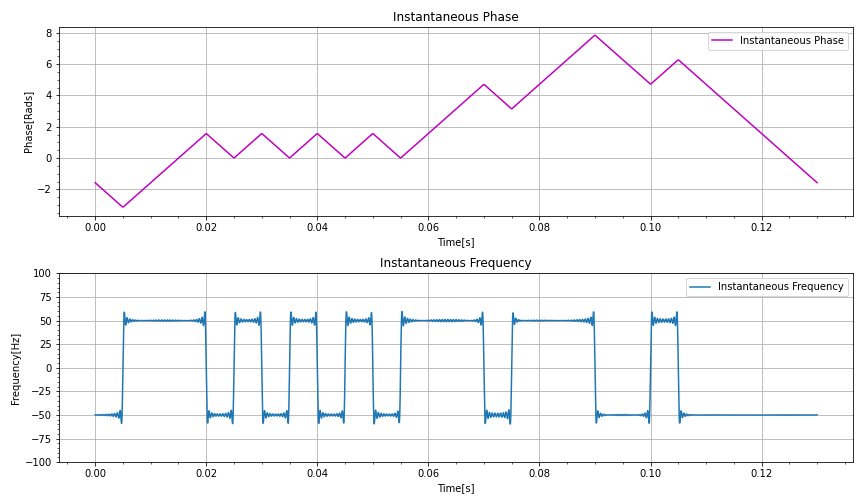
\includegraphics[width = \textwidth]{figs/sim/simDemod.png}
    \caption{Demodulated Simulation Signal.}
    \label{fig:simDemod}
\end{figure}

\pagebreak
\subsection{Additive Noise}
In order to allow the simulation to most accurately represent the real world situation APD's have been generated from the real world data. A scaling factor was required in order to provide an accurate result. As illustrated by the results in section \ref{sec:noiseEst}. Depending on which transmitter is being simulated defines the APD that is used to support it. Looking at the GQD transmitter the APD for this is shown by figure \ref{fig:apdcdf}, including the CDF which is of particular interest because this is what allows for much simpler computation.

\begin{figure}[h!]
    \centering
    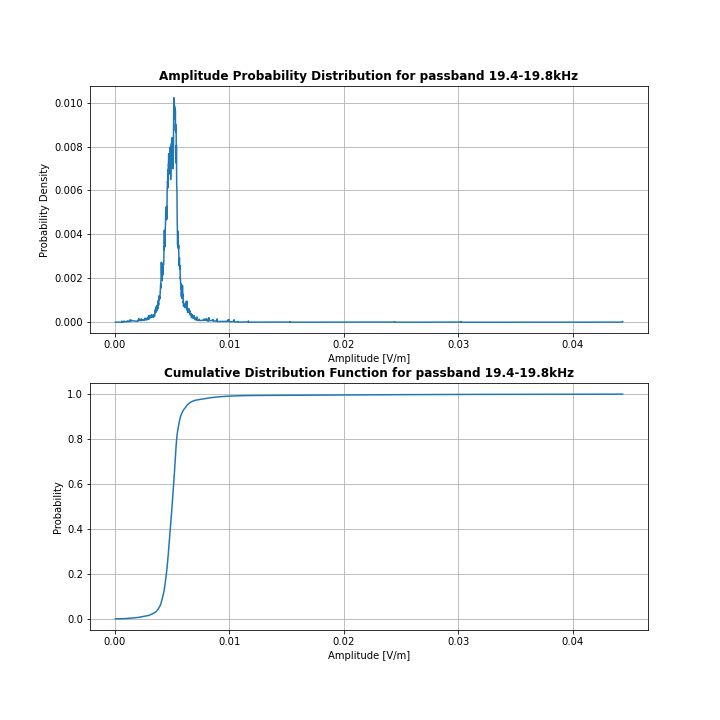
\includegraphics[width = \textwidth]{figs/sim/apdcdf.png}
    \caption{APD and CDF for GQD Transmitter}
    \label{fig:apdcdf}
\end{figure}

In order to match the noise signature from the recorded data, a random amplitude is selected and then combined with a random phase in order to create a complex point to be added to the signal. These points are added in bursts of 500 - 10000 samples which is 500\si{\nano\second} to 20\si{\milli\second}, with $n$ bursts in each signal. This is to represent the two different natures of previously established interference.

\pagebreak
\subsection{Validation}
The full simulation involved combining the ideal simulated waveform with a simulated noise waveform. The time series is shown by figure \ref{fig:timeseries} and the demodulated signal is shown by figure \ref{fig:fullsimDemod}. This particular example illustrates an attempt to simulate the transmitter GQD, this has been chosen as it has the lowest SNR. Comparing the recovered baseband signal to figure \ref{fig:AnthornDemod} it can be shown on the surface to exhibit similar properties and an SNR of -4dB. The simulation represents a random bit sequence and a gain on the APD value for additive noise of 5 for burst greater than 5000 samples and 10 for bursts less than 5000 samples.

Figure \ref{fig:polar} shows these signals in the complex plane, as there is a certain stochastic nature to lightning interference. However these three plots do illustrate how the lightning effects the points at which the symbols changes in reality, and how the lightning effects how the symbols are detected. As it pulls away from the phasor and then returns.


\begin{figure}[h!]
    \centering
    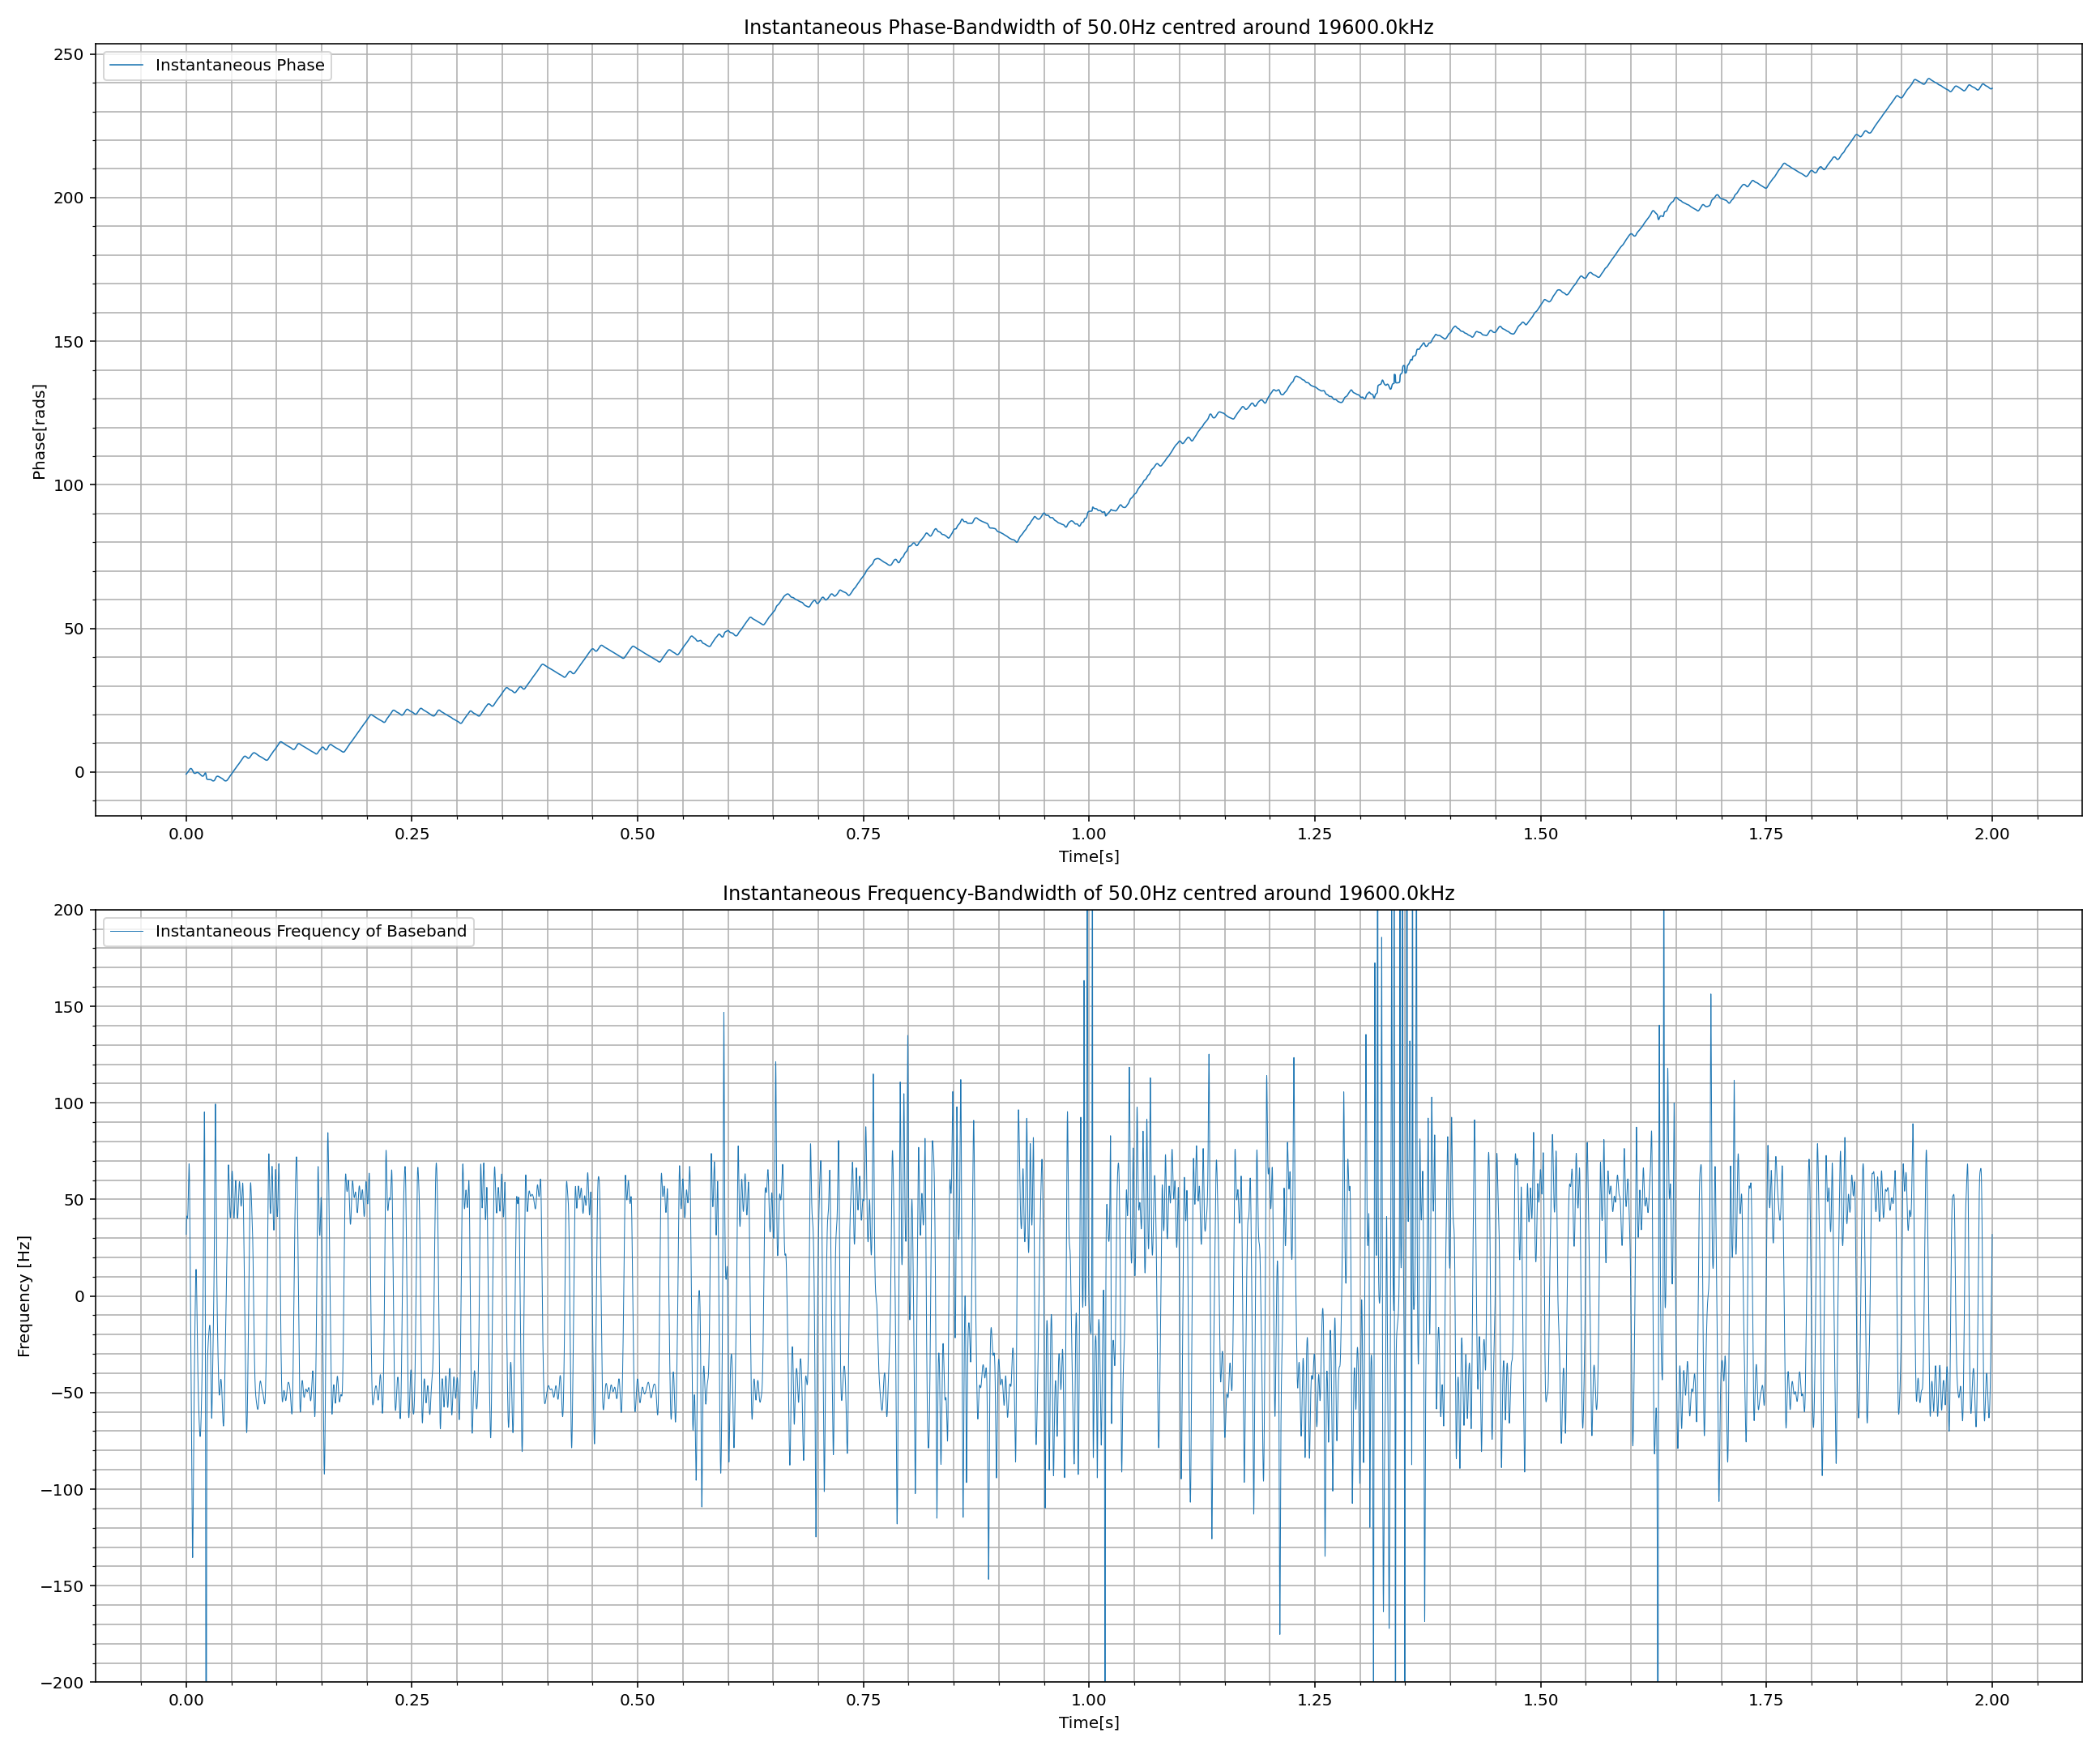
\includegraphics[width=0.8\textwidth]{figs/sim/veri/GQDver.png}
    \caption{\centering Instantaneous Phase and Frequency for transmitter GQD extracted from real data}
    \label{fig:AnthornDemod}
\end{figure}
\begin{figure}[h!]
    \centering
    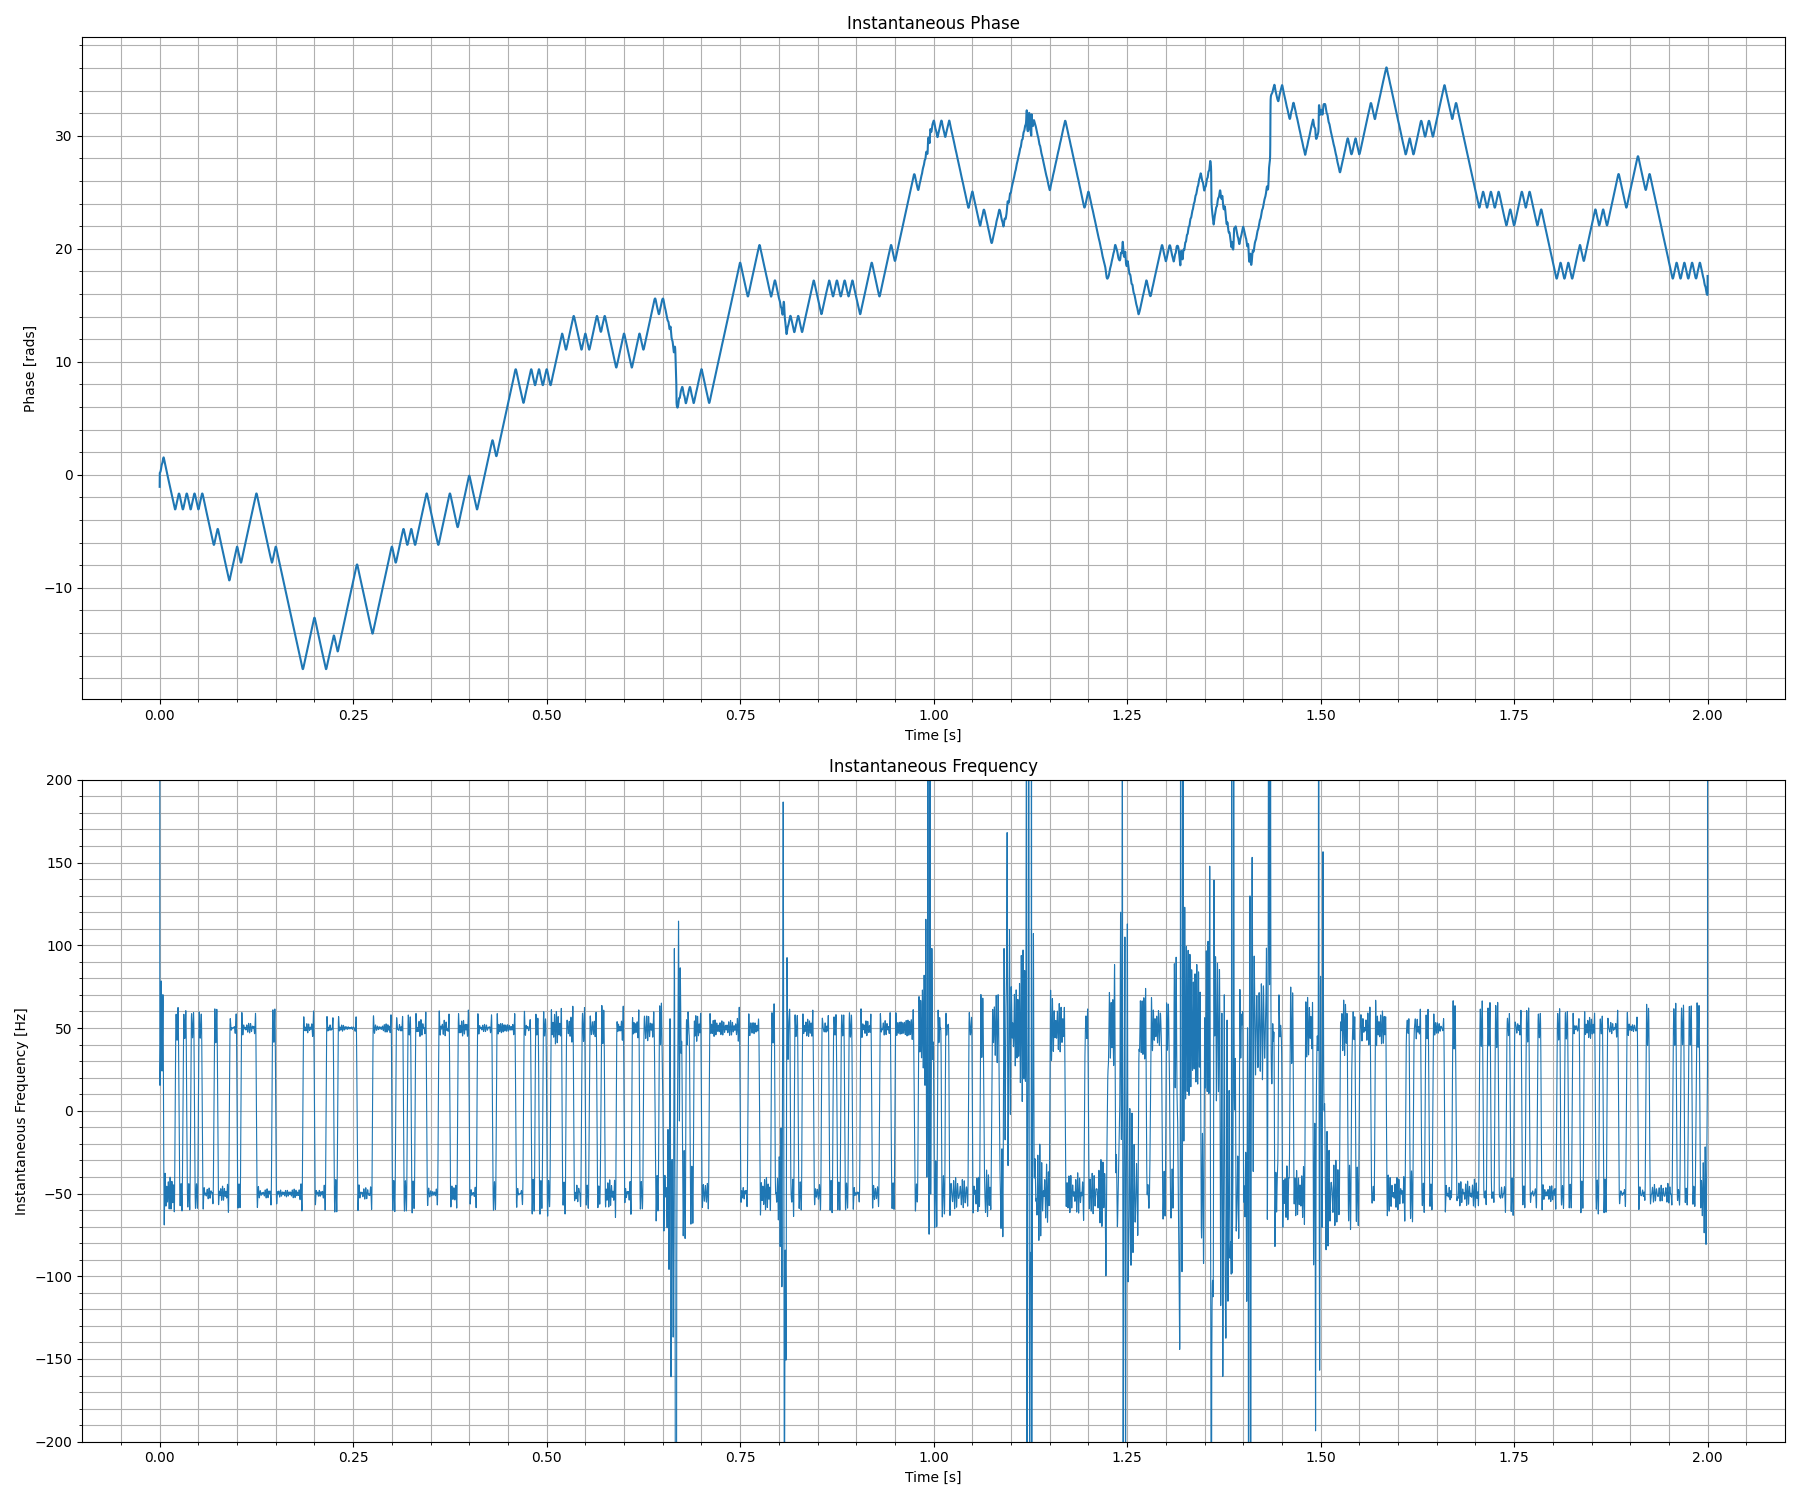
\includegraphics[width = 0.8\textwidth]{figs/sim/veri/GQDfreq.png}
    \caption{\centering Instantaneous Phase and Frequency for simulated GQD}
    \label{fig:fullsimDemod}
\end{figure}
\begin{figure}[H]
    \centering
    \begin{subfigure}[b]{0.4\textwidth}
        \centering
        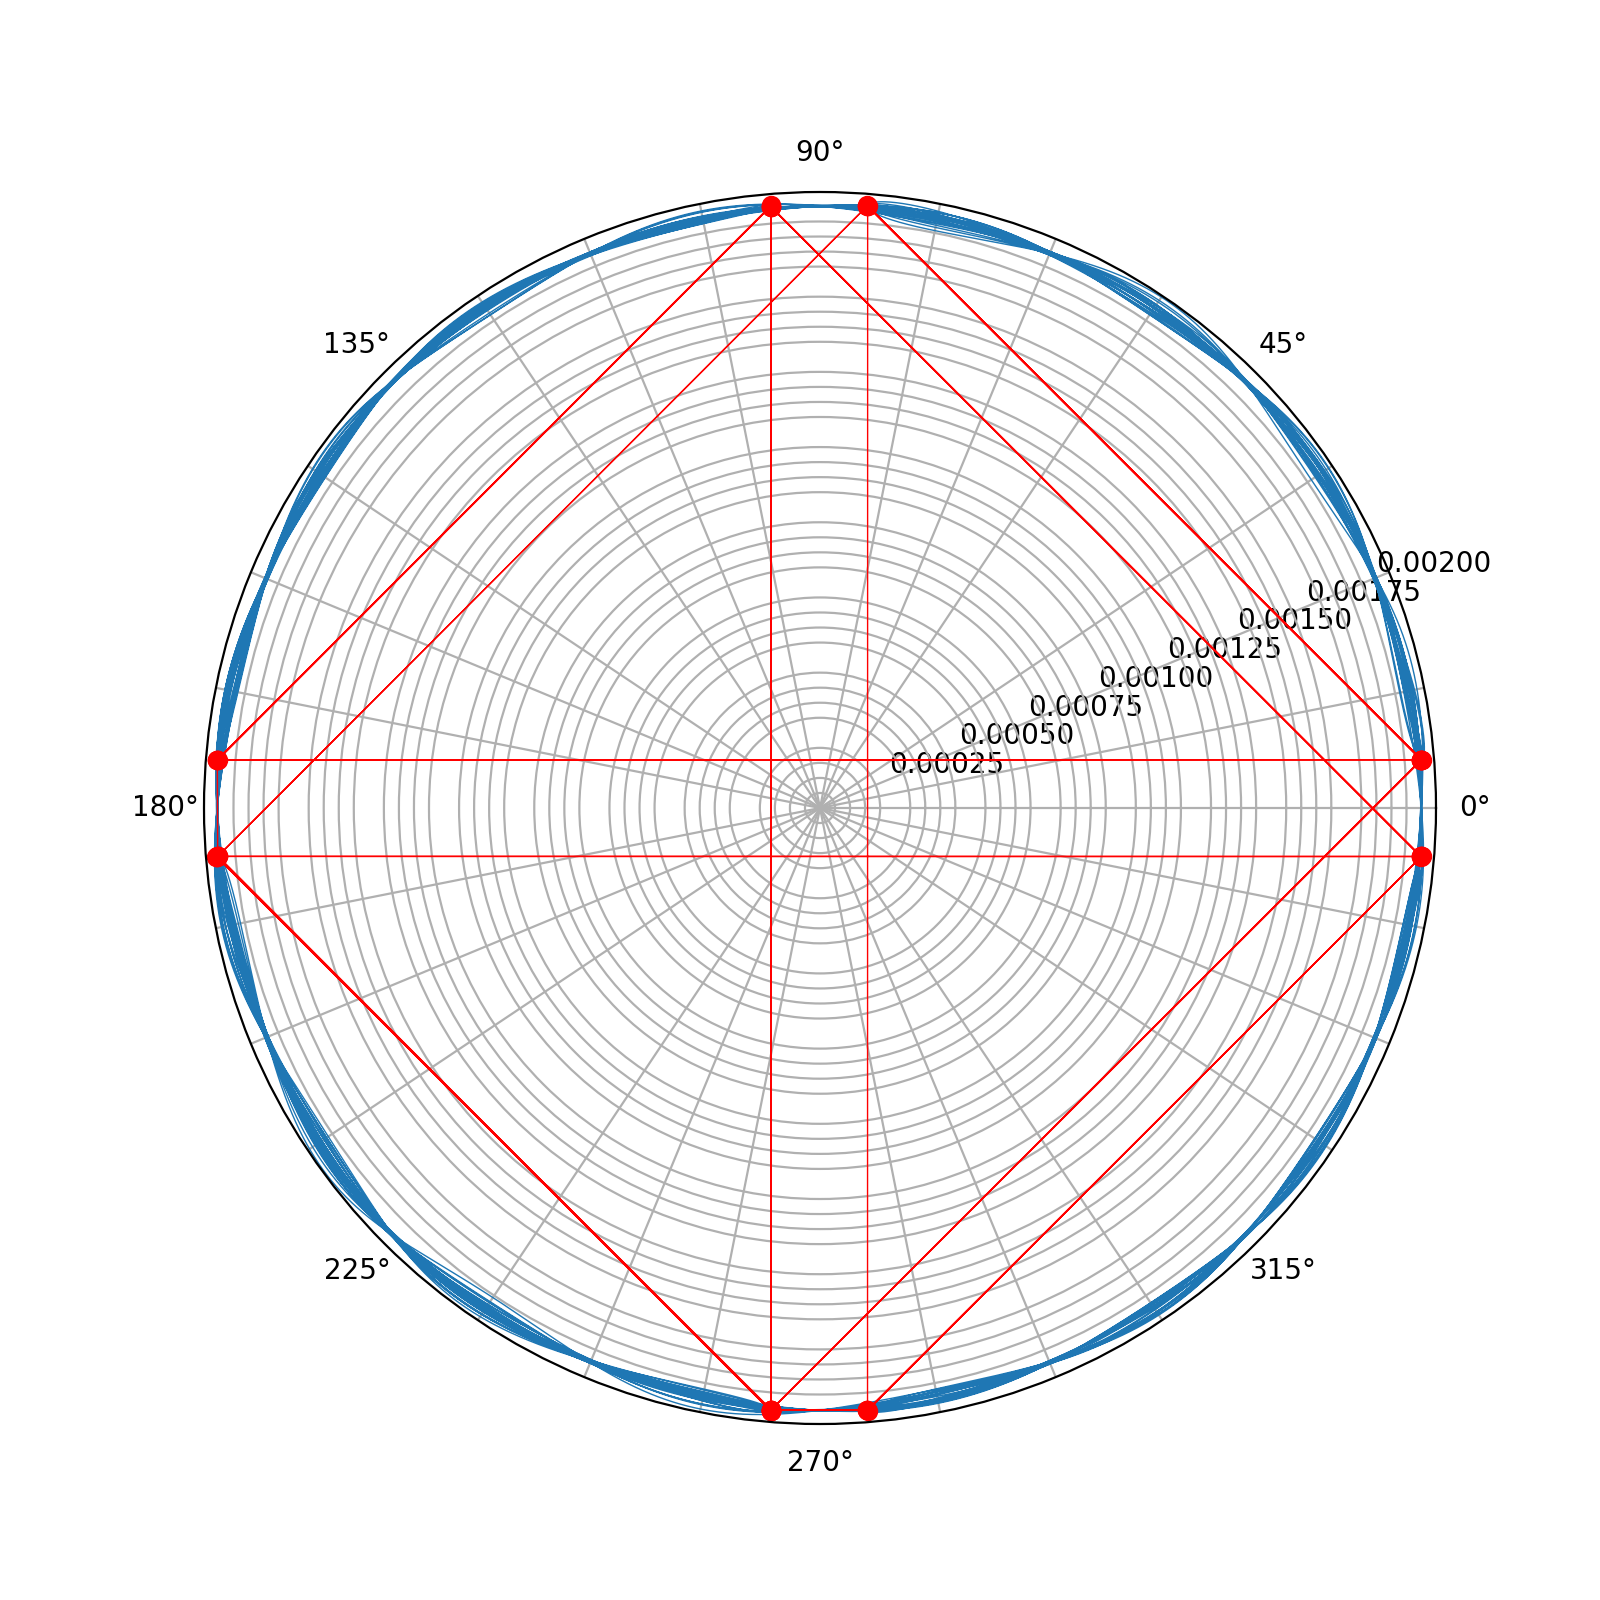
\includegraphics[width = \textwidth]{figs/sim/veri/polar_control.png}
        \caption{Polar Plot of Ideal MSK signal}
        \label{fig:polarcontrol}
    \end{subfigure}
        \begin{subfigure}[b]{0.4\textwidth}
        \centering
        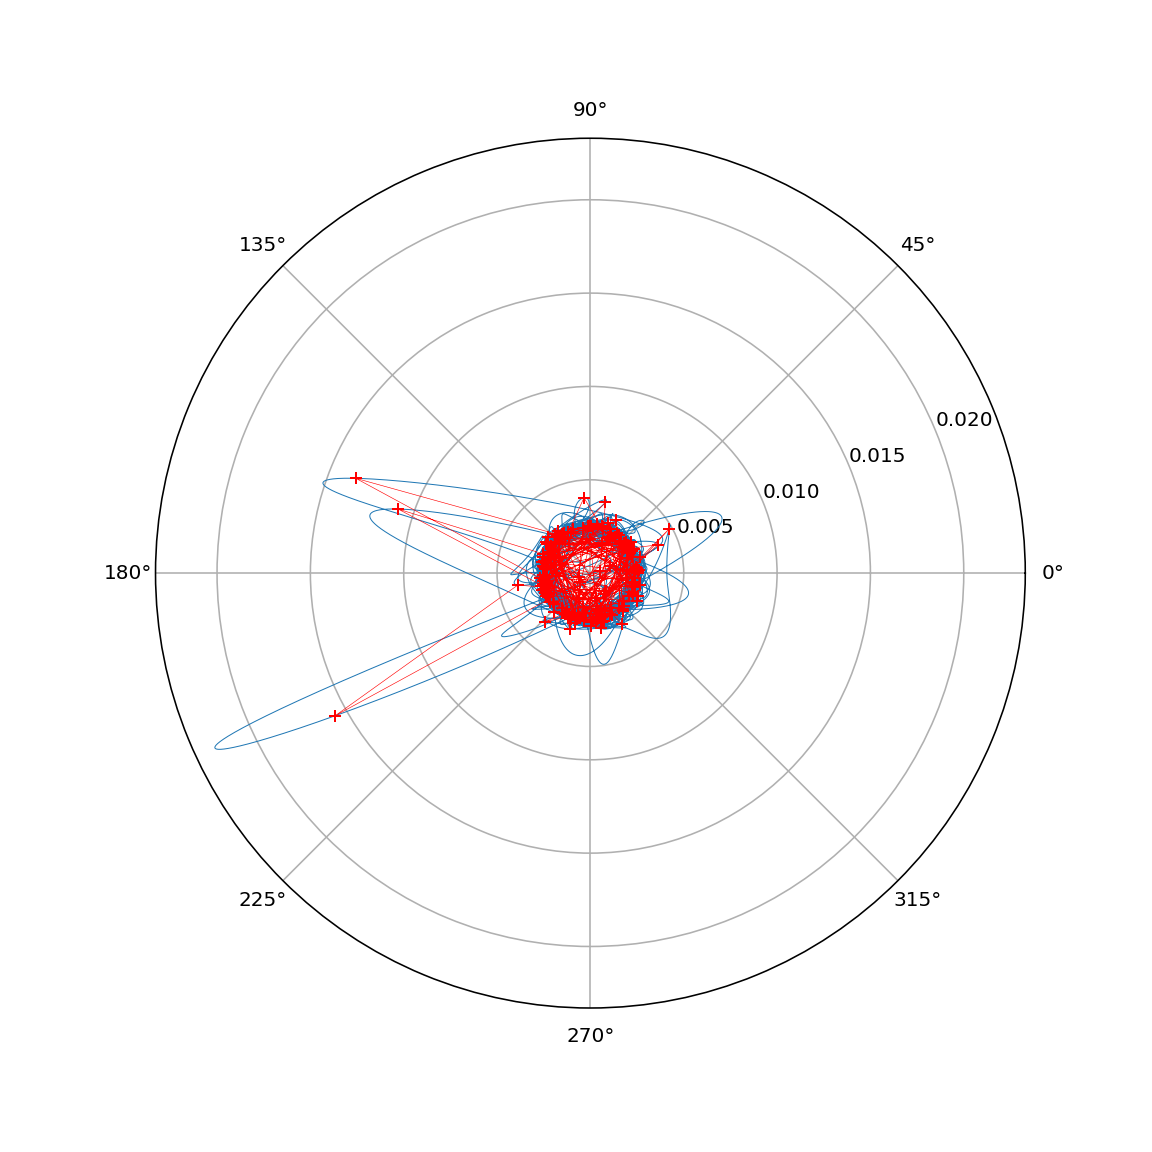
\includegraphics[width = \textwidth]{figs/sim/veri/polarreal.png}
        \caption{\centering Polar Plot of Signal from transmitter GQD}
        \label{fig:polarreal}
    \end{subfigure}
        \begin{subfigure}[b]{0.4\textwidth}
        \centering
       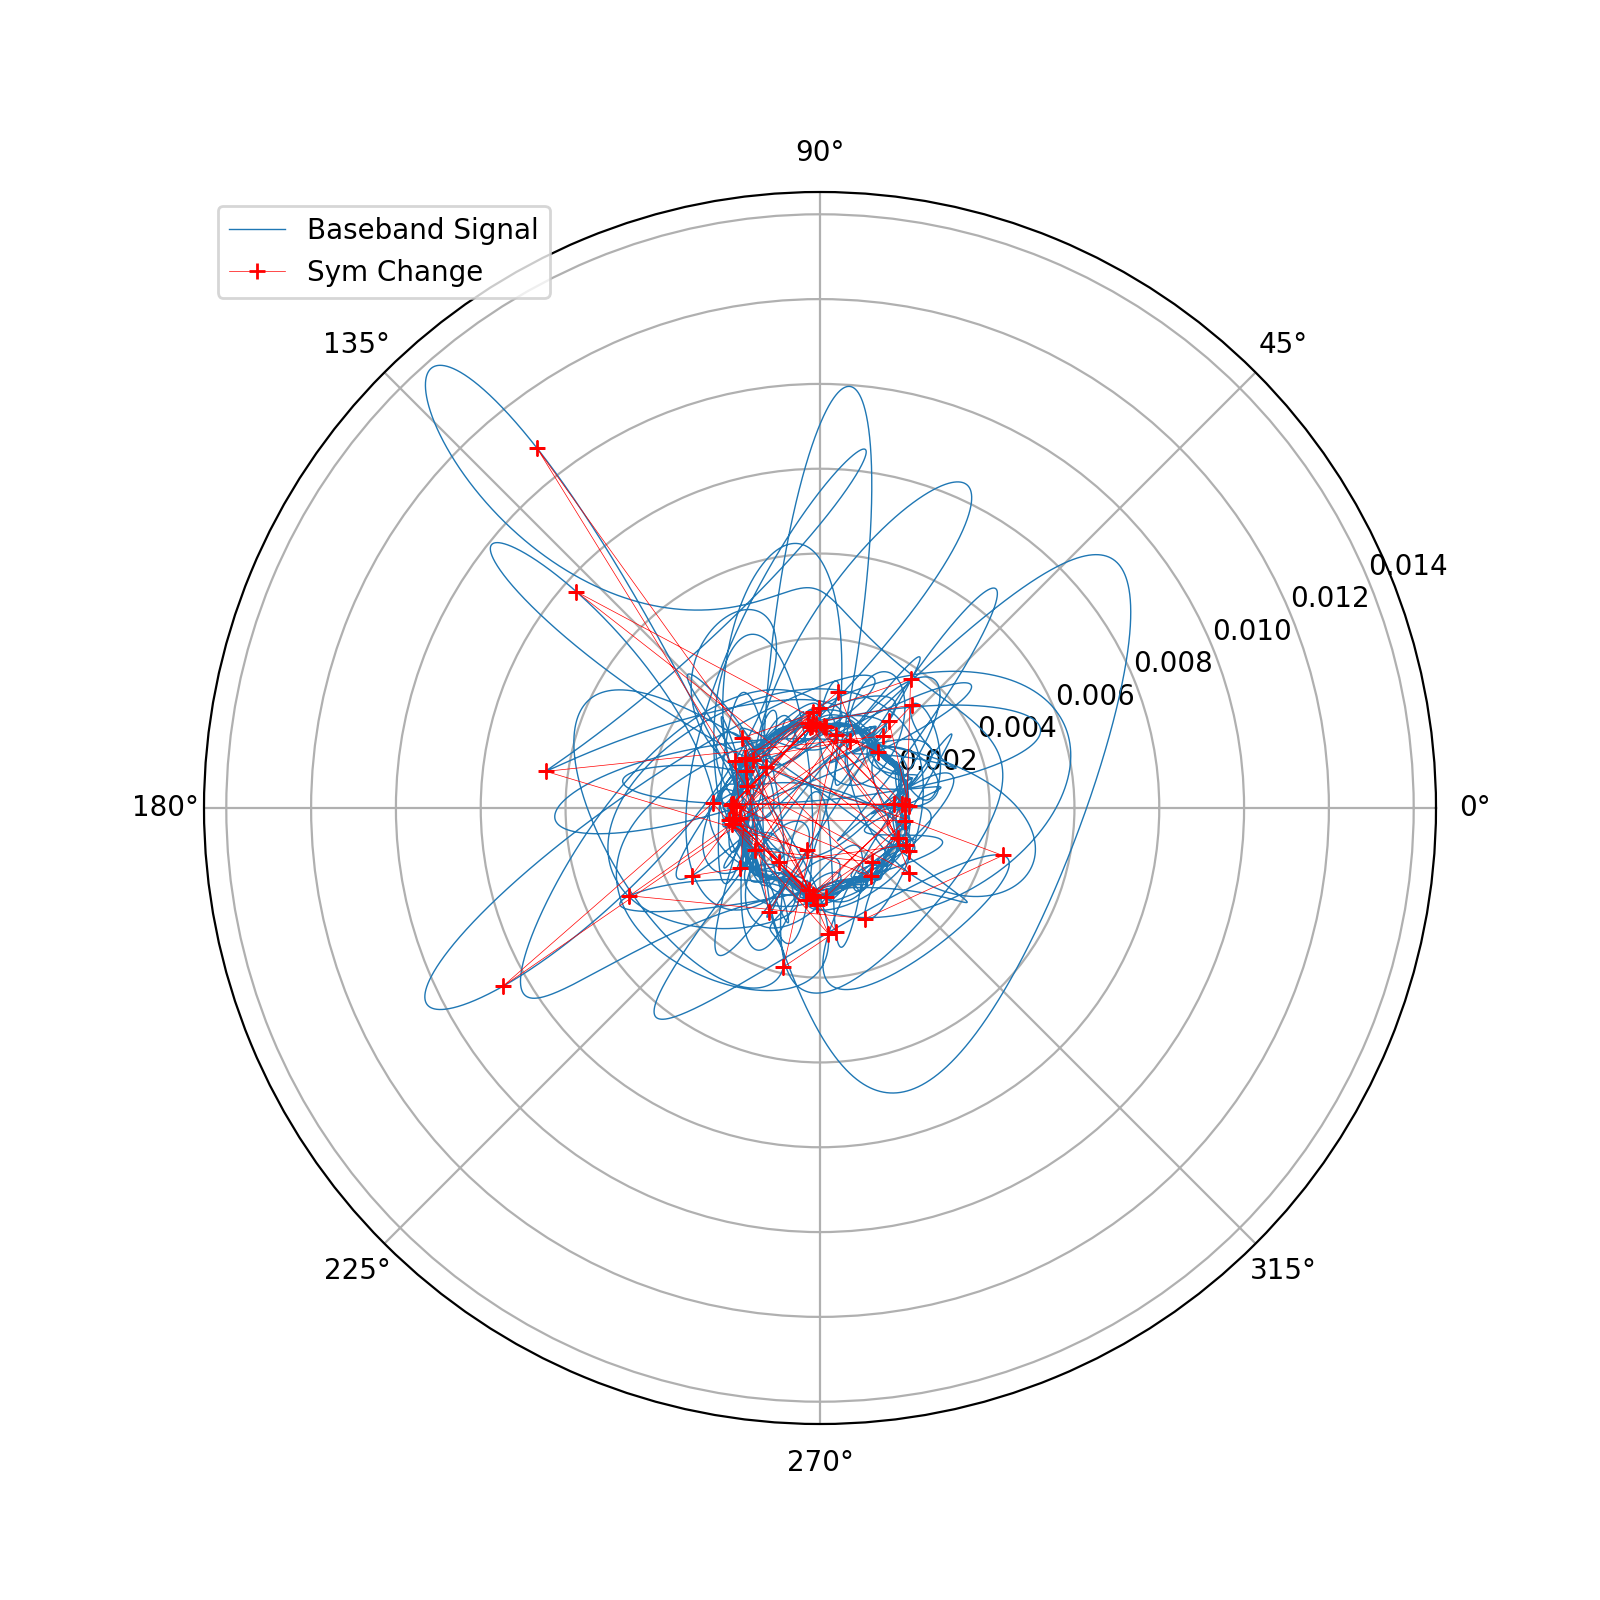
\includegraphics[width = \textwidth]{figs/sim/veri/PolarSim.png}
        \caption{Polar Plot of Simulated Signal}
        \label{fig:polarSim}
    \end{subfigure}
    \caption{Ideal,Recorded and Simulated Signals in the Complex Plane}
    \label{fig:polar}
\end{figure}


\pagebreak
\section{Symbol Recovery}
Following on from an intensive investigation which is summarised in section \ref{sec:sigChar}. Two possible methodologies were identified to recover the message symbols from the received signal.

\begin{itemize}
    \item Image based: Using narrowband Spectrograms in order to develop an image recognition tool to recover the original bits.
    \item Geometric: Effectively a graph based system using known properties of the carrier wave in order to estimate the symbols based of the instantaneous phase and frequency.
\end{itemize}

Although there are significantly powerful image processing tools that may be able to help with this problem broadband interference can have a significant effect on spectrograms and then the quality of the image becomes limited twofold. Firstly a key factor can be that the color map may not contain sufficient colors to allow the lightning to be discriminated and secondly depending on what is surrounding the transmitter the signal processing uncertainty principal comes into play, meaning that a compromise of either time or frequency resolution is required. This is exemplified by figure \ref{fig:gqdspect} as although the frequency changes are clear the two limiting factors are overwhelming clear, firstly because the time resolution is greater than $T_b$ for a signal with 200Hz bandwidth there will not be enough discrete symbols visible. Secondly because the power of the lightning impulse is much greater than the power of the transmitter the lightning event will in all effect blank out each time interval that it is present in. As good practice tends to use a sampling frequency an order of magnitude greater than the frequency of interest, therefore for this particular example the signal could be downsampled to 250\si{\kilo\hertz}, which would allow for an improved time resolution. Equally this could be achieved by using shorter sample sizes for the spectrogram.

\begin{figure}[h!]
    \centering
    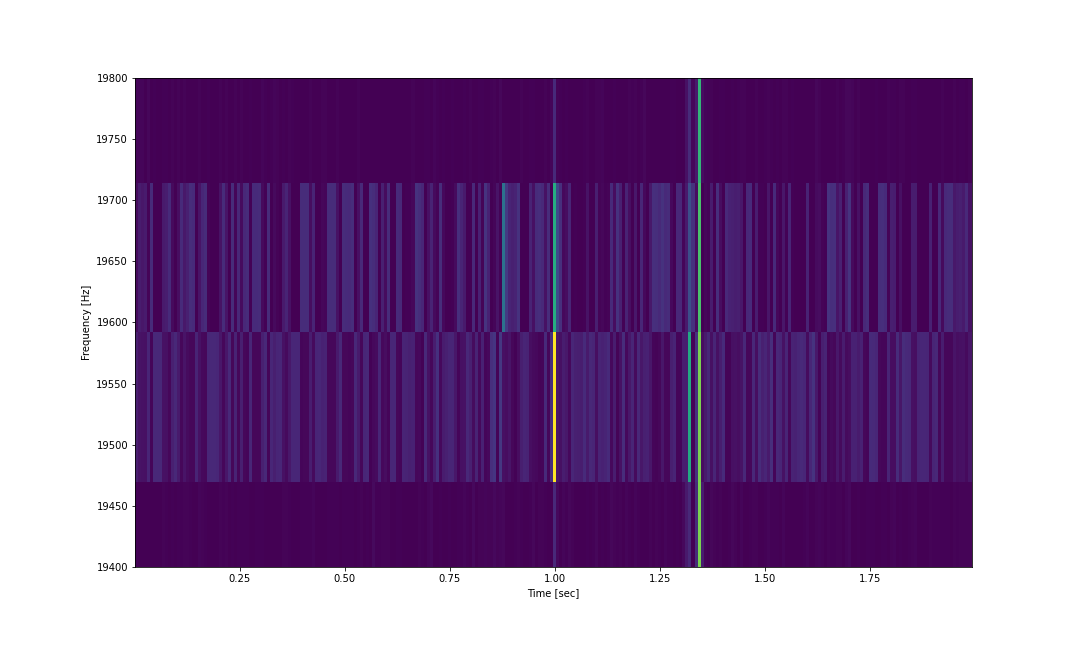
\includegraphics[width = \textwidth]{figs/sim/symRecovery/GQDSpectrogram.png}
    \caption{Spectrogram of Transmitter GQD with $\Delta t = 7\si{\milli\second}$}
    \label{fig:gqdspect}
\end{figure}

\subsection{Algorithm Design}

The basis to go for essentially a graphical approach using the principles of the differential of the phase is considered optimal, especially for the example data because it is recorded with such a small time resolution this can be utilised. As there are known quantities that can be extracted from the signal. The basic algorithm works simply on differentials. The Instantaneous Phase is an integrated measurement equivalent to displacement, because the frequency changes direction everytime there is a symbol change this represents a turning point in the phase. The first differential of the phase is frequency and hence a crossing of the zero axis will occur. This symbol change of the instantaneous frequency is the basis of the extraction algorithm. From a received signal it is possible to calculate the transmission bandwidth from the variation in instantaneous frequencies. Referring again to Appendix X the information shown in table \ref{tab:transinfo} can be inferred in particular the bandwidth from which $T_b$ can be calculated using equation \ref{eq:tb}. By combining with the $f_s$ using equation \ref{eq:Ns} which calculates the number of samples per symbol. 

\begin{subequations}
\begin{equation}
    T_b = 1/BW
    \label{eq:tb}
\end{equation}
\begin{equation}
    N_s = f_S \times T_b
    \label{eq:Ns}
\end{equation}
\end{subequations}

\begin{table}[h!]
    \centering
    \begin{tabular}{l|l|c|c}
    \textbf{Callsign} & \textbf{Location} & \textbf{Centre Frequency
    $f_c$}[kHz] & \textbf{Bandwidth} [Hz] \\
    \hline
    \textbf{GQD} & Anthorn, UK & 19.6 & 200 \\
    \textbf{HWU} & Saint-Assise, France & 20.9 & 200 \\
    \textbf{GZQ} & Skelton, UK & 22.1 & 100 \\
    \textbf{DHO38} & Rhauderfehn, Germany & 23.4 & 200 \\
    \textbf{NAA} & Cutler, Maine USA & 24 & 200 \\
    \end{tabular}
    \caption{Transmitter Information}
    \label{tab:transinfo}
\end{table}

\begin{figure}[h!]
    \centering
    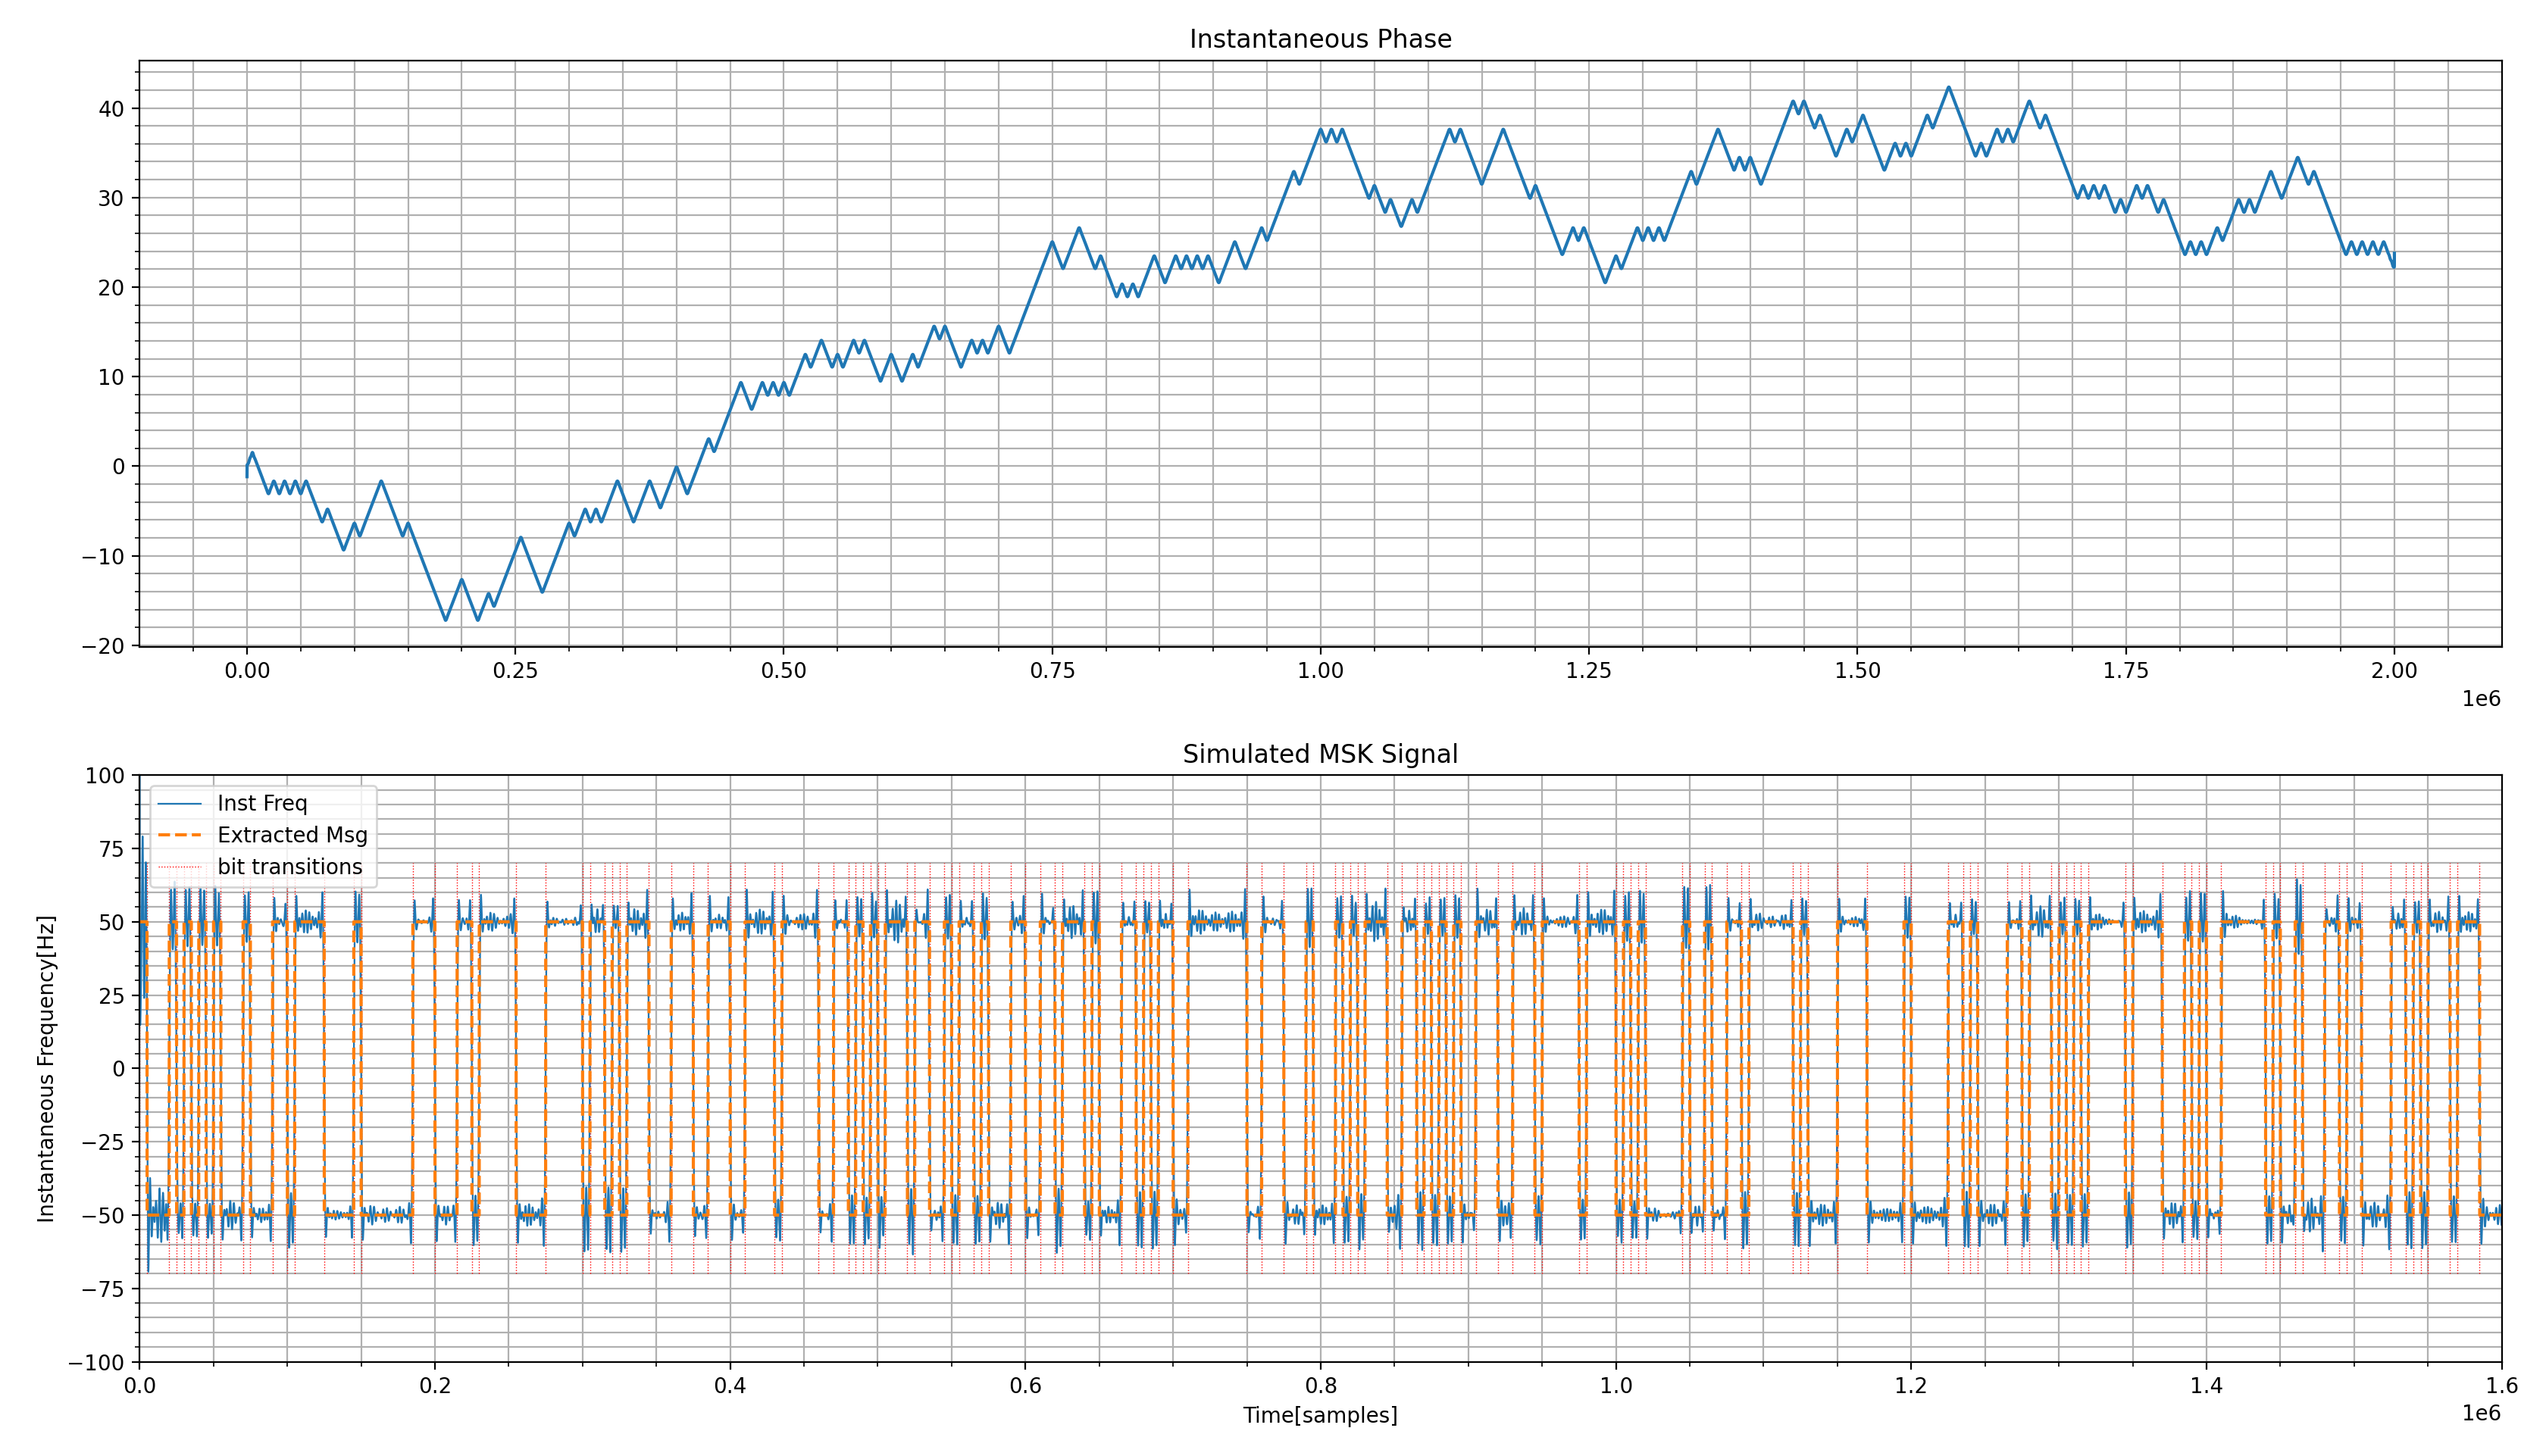
\includegraphics[width = \textwidth]{figs/sim/symRecovery/ideal_demod.png}
    \caption{Bit recovery from Ideal MSK signal}
    \label{fig:idealBits}
\end{figure}

For an ideal coherent signal these crossing of the time axis should occur an integer multiples of the value $N_s$, depending how many consecutive symbols with the same sign there are. Such a signal is shown by figure \ref{fig:idealBits} where this method recovers the entire signal. As it is clear that each of the transition lines up with the index returned by the algorithm, and the square wave of the extracted signal matches exactly.

\subsubsection{Algorithm}
\begin{enumerate}
    \item Find all crossings of the time axis in the instantaneous frequency using a sign change technique. Recording the index of each crossing.
    \item Iterate through all indexes, calculate the time difference between each index to determine if it is long enough for a symbol. A threshold may be applied for example: $\Delta t > 0.8T_b$.
    \item Check the gradient of the crossing at the index:
    \begin{itemize}
        \item Positive Gradient is a transition of 0 to 1.
        \item Negative Gradient is a transition of 1 to 0.
    \end{itemize}
    \item The number of symbols for the given interval is given by equation \ref{eq:nbits}.
    \begin{equation}
        N_{\text{bits}} = \frac{\Delta t}{N_s}
        \label{eq:nbits}
    \end{equation}
    \item At each instance compare the number of bits compiled against the elapsed time and if necessary insert additional bits to ensure that the extracted signal has the correct number of elements.
    \item After the last crossing calculate the sign of the last sequence and apply equation \ref{eq:nbits}.
\end{enumerate}




\subsection{Application to Real Signal}
\begin{table}[h!]
    \centering
    \begin{tabular}{l|l}
    Callsign & BER           \\
    \hline
    GQD      & $e^{-1.69}$  \\
    HWU      & $e^{-17.74}$ \\
    GZQ      & $e^{-13.86}$ \\
    DHO38    & $e^{-3.91}$  \\
    NAA      & $e^{-4.38}$ 
    \end{tabular}
    \caption{Estimated Bit Error Rate for VLF Transmitters}
    \label{tab:BER Real}
\end{table}

In it's most basic form the results of this algorithm when applied to the 5 signals in the noisy data are shown by table \ref{tab:BER Real}. Figure \ref{fig:snrwins} shows these values plotted against the respective SNR for each transmitter, with a crude best fit line plotted to show the trend. The DHO transmitter was eliminated from this calculation because it is clearly a data outlier, this is likely because the SNR calculation is not accurate in this instance. A likely reason for this referring back to section \ref{sec:sigChar} is that due to the clipping in the data acquistion there appears to be less noise present in this signal. However the bit loss associated with this signal suggests otherwise. 

It is important to also note that because these signal contain 400 bits each with the exception of GZQ which has half the bandwidth so therefore only transmits 200 bits. Any BER value less than $10^{-6}$ for this number of bits corresponds to complete recovery of the original signal.

Comparing against figure \ref{snr:charmy} which as previously mentioned has a minimal noise content. This signal only contain four active transmitters however all four transmitters are achieving full bit recovery.

\begin{figure}[h!]
    \begin{subfigure}[b]{0.5\textwidth}
    \centering
    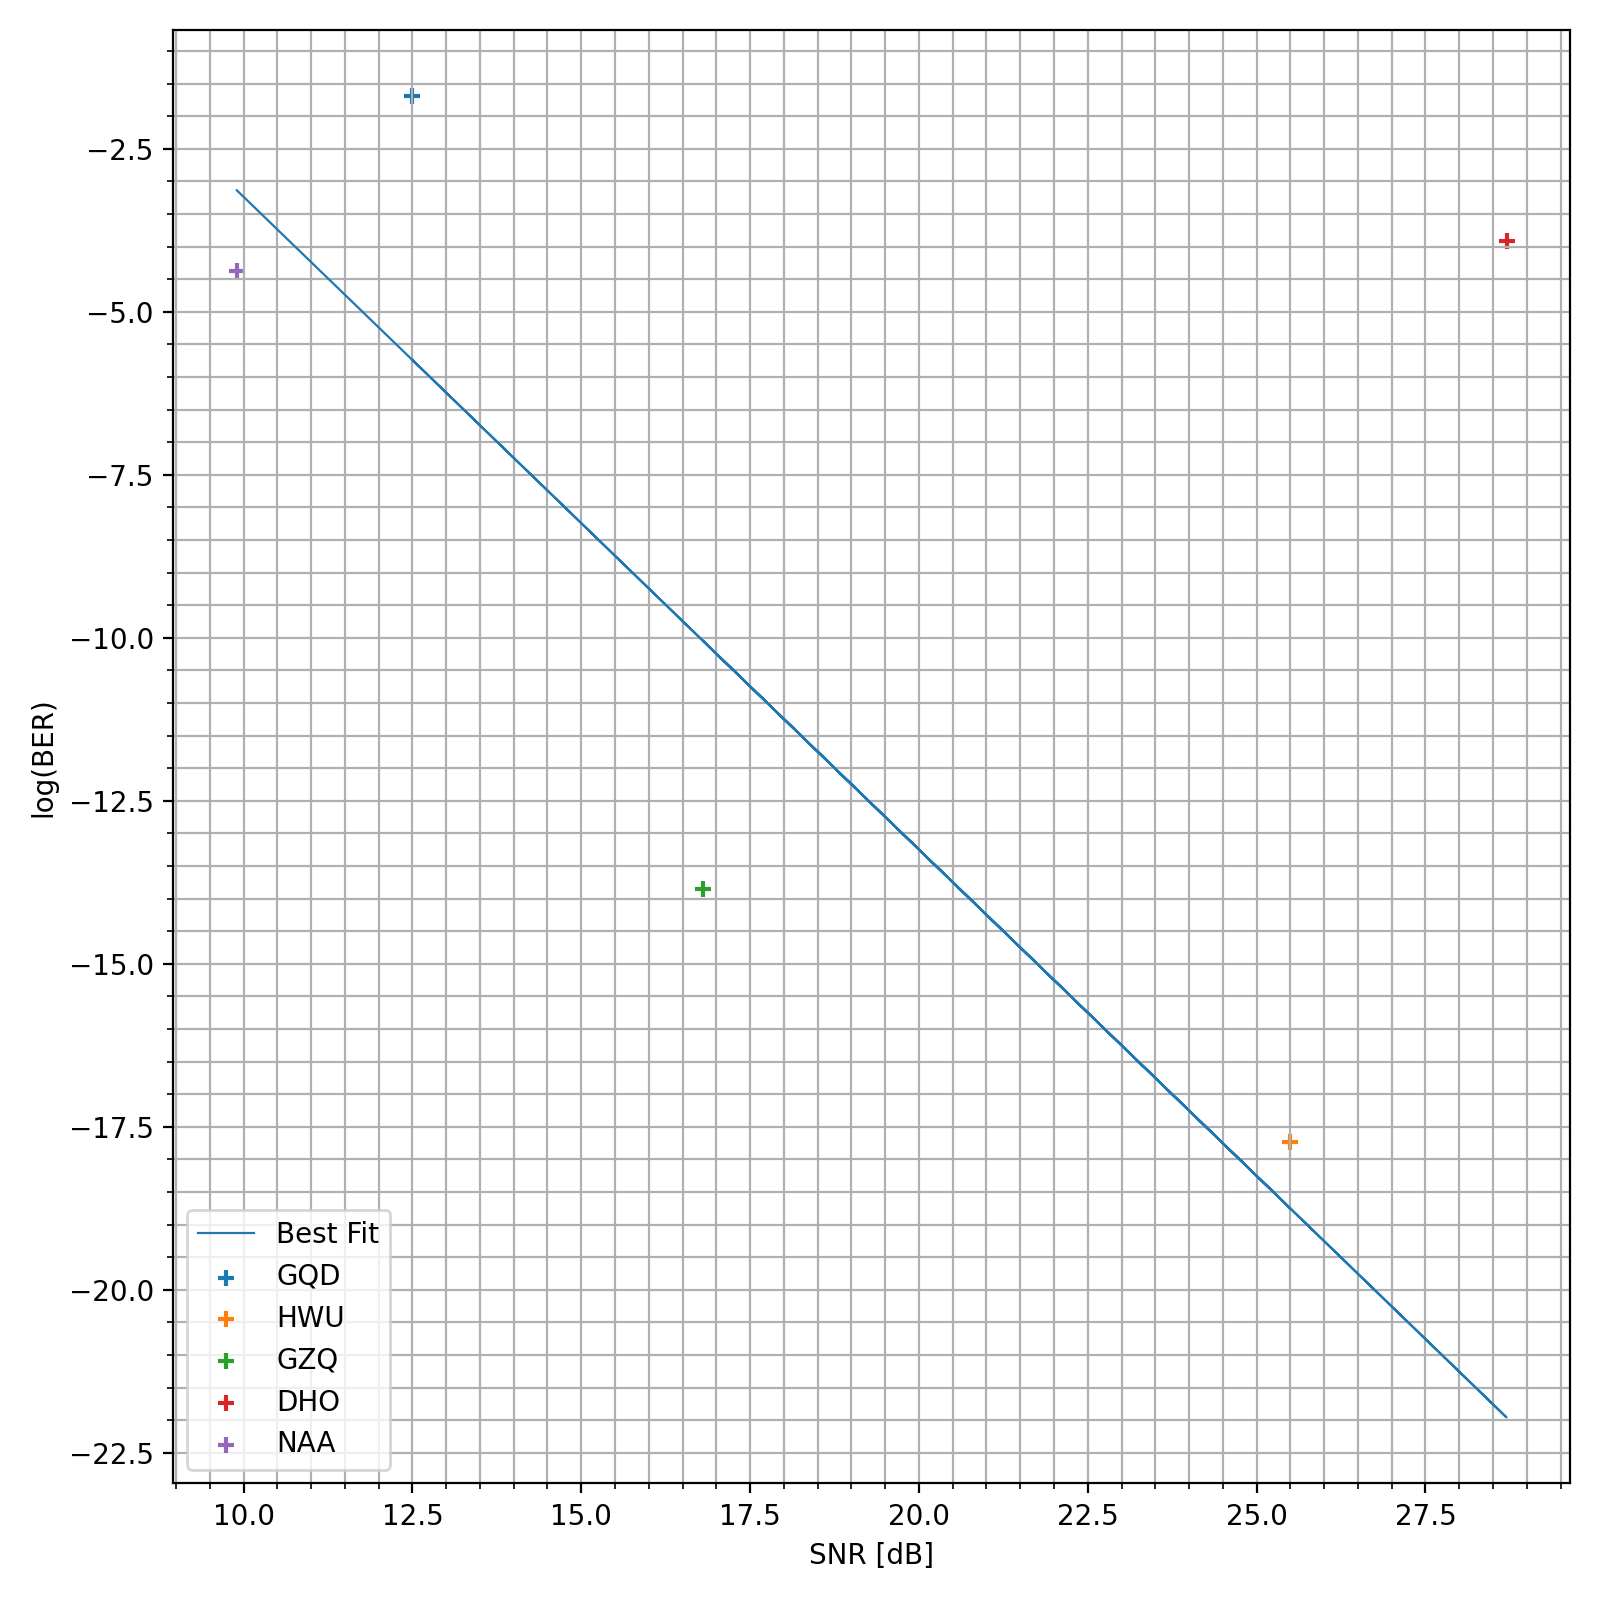
\includegraphics[width = \textwidth]{figs/sim/symRecovery/snrvber_real.png}
    \caption{SNR vs BER for High Noise Data}
    \label{fig:snrwins}
    \end{subfigure}
    \begin{subfigure}[b]{0.5\textwidth}
    \centering
    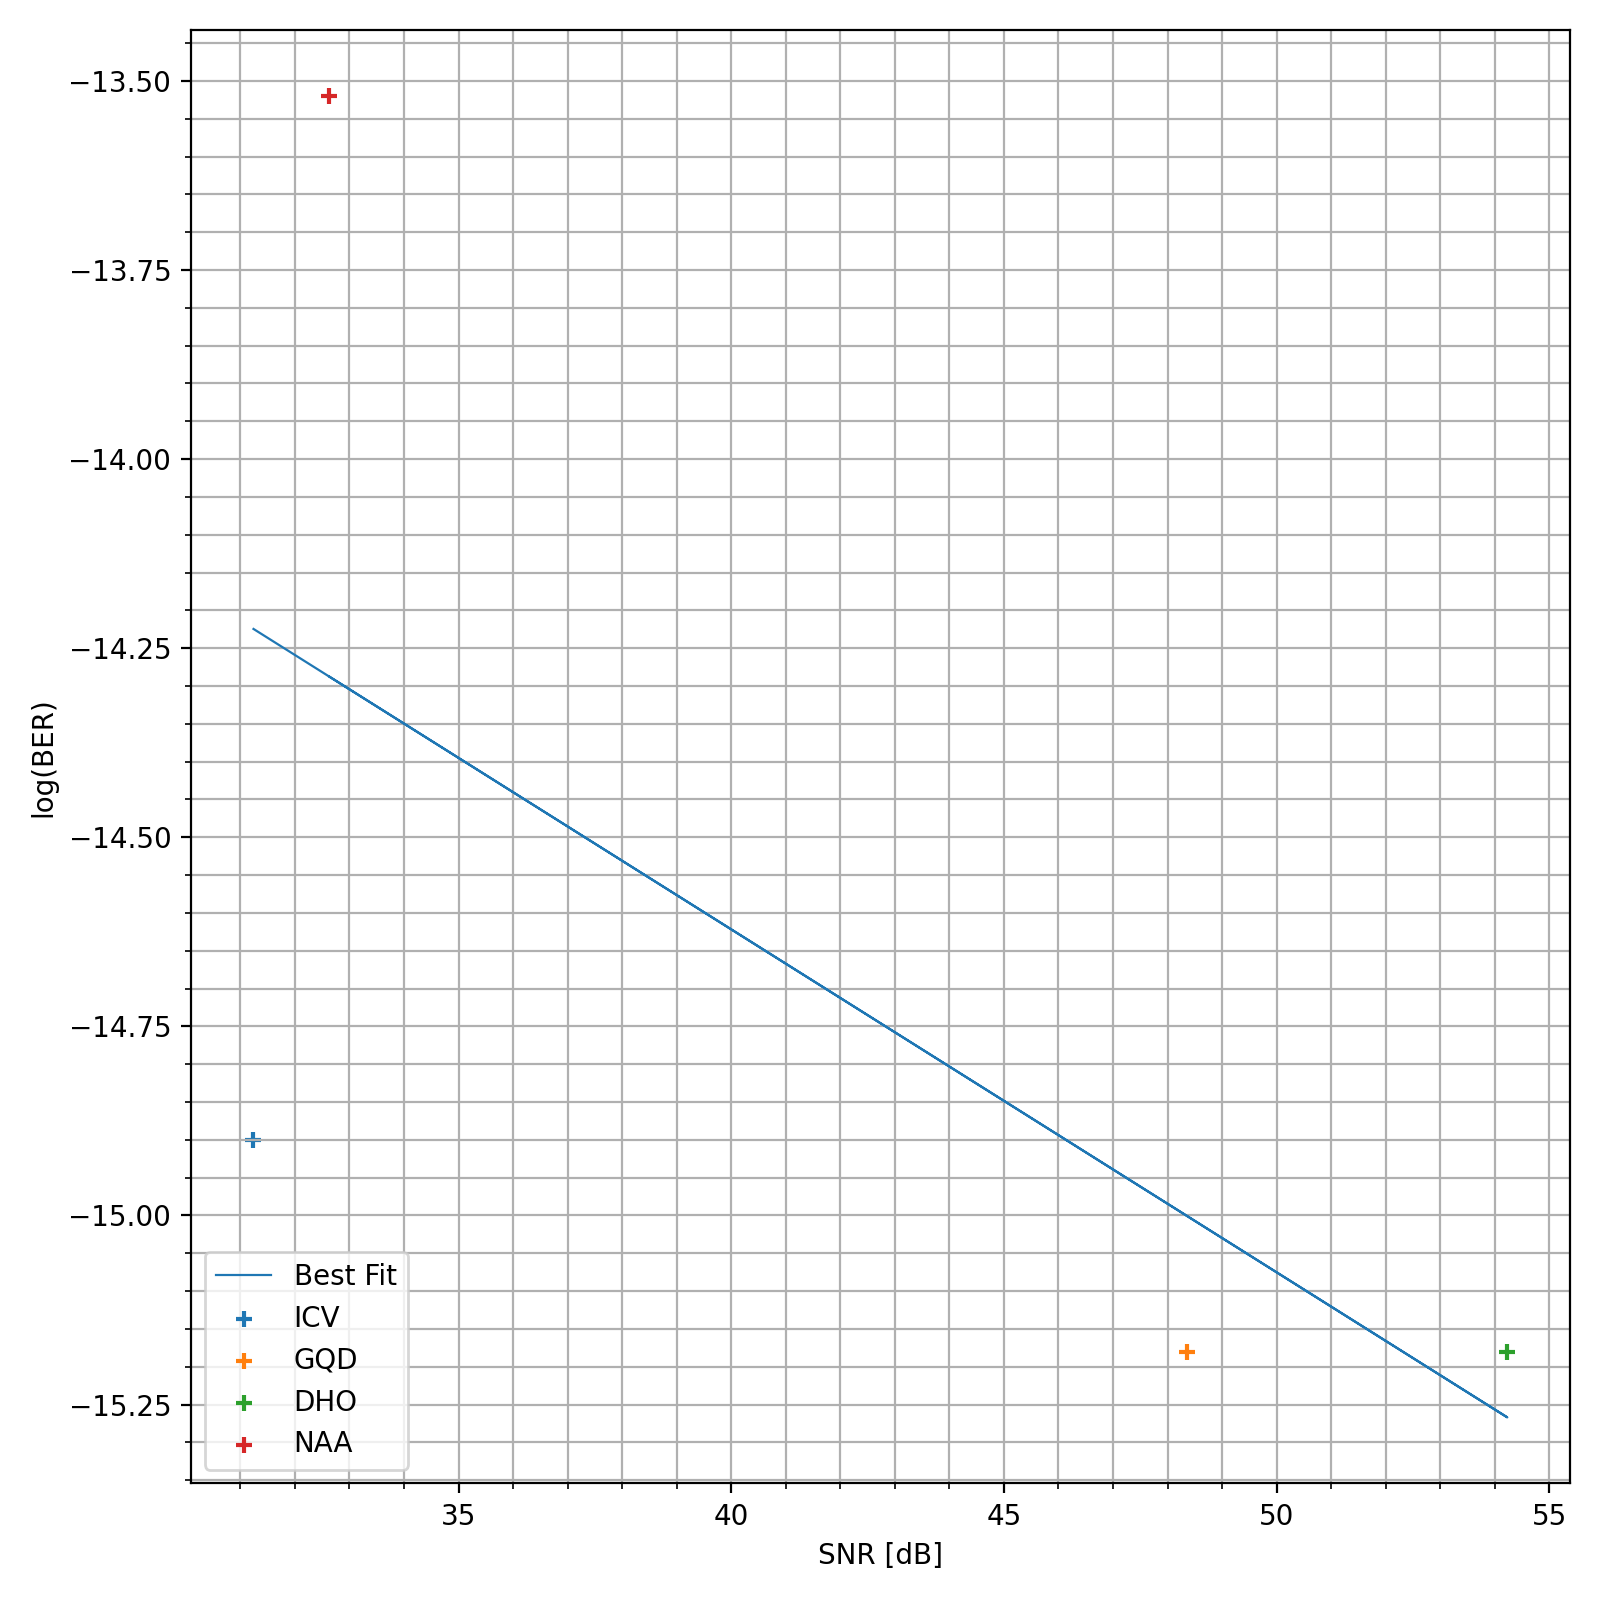
\includegraphics[width = \textwidth]{figs/sim/symRecovery/snrvber_real_charmy.png}
    \caption{SNR vs BER for Low Noise Data}
    \label{snr:charmy}
    \end{subfigure}
    \caption{}
\end{figure}
\pagebreak
\subsection{Application to Simulated Signals}

Table \ref{tab:simresults1} shows the results of three random simulations for 4 of the 5 transmitters present. DHO has not been simulated because the quality of the data for this transmitter appears to differ from expected values. The BER shown represent a bit loss of between 1 and 4 over the total length of the signal.


\begin{table}[h!]
\centering
\begin{tabular}{l|l|c|c|c|c|c|c}
         &                        & \multicolumn{2}{c}{1} & \multicolumn{2}{|c}{2} & \multicolumn{2}{|c}{3} \\
         \hline
Callsign & Centre Frequency $f_c$ & SNR    & BER          & SNR    & BER          & SNR    & BER          \\
\hline
GQD      & 19.6                   & -26.2  & $e^{-5.99}$ & -31.6  & $e^{-4.61}$ & -30.2  & $e^{-4.61}$ \\
HWU      & 20.9                   & -30.1  & $e^{-5.30}$ & -20.4  & $e^{-5.30}$ & -25.7  & $e^{-5.30}$ \\
GZQ      & 22.1                   & -21.9  & $e^{-5.30}$ & -23.8  & $e^{-5.30}$ & -34.1  & $e^{-5.30}$ \\
DHO38    & 23.4                   & -      & -            & -      & -            & -      & -            \\
NAA      & 24                     & -31.0  & $e^{-4.89}$ & -28.6  & $e^{-4.61}$ & -29.2  & $e^{-5.30}$
\end{tabular}
\caption{Simulation Results}
\label{tab:simresults1}
\end{table}

Figure \ref{fig:noisefreq} shows the results of demodulation for an ideal MSK signal that has been corrupted by noise based off the transmitter at 19.6 kHZ. The noise signal in question is shown in figure \ref{fig:noiseamp}. In both figures the points where there is a missed transition is illustrated, by looking at the noise signal it is clear that the transitions occur at the end of a lightning event shown by the amplitude pulses. 

This is where the slight randomness of the problem is highlighted. This simulation contains 20 'lightning' pulses however there are only 3 missing bit transitions, there are however the correct number of bits in the signal. This is likely due to lightning event introducing a resultant phase at an obtuse angle relative the phase of the transmitter which results in an apparent symbol change. Depending on where the error often occurs at a transition point close to the edge of a burst. 

Because of how the algorithm iterates through the data and that the effect of the noise may move the zero crossing. At each crossing the algorithm checks that it has the correct number of bits for the elapsed time. As a result if the lightning creates an instantaneous phase within $0.8T_b$ of an actual crossing then this may result in a sequence being shortened and an additional bits being added at the next crossing due to the apparently longer interval between crossings. 

An additional error is missing a single symbol change within a long sequence of one symbol.

\begin{table}[h!]
    \centering
    \begin{tabular}{c|c|c}
        $f_c$[kHz]&SNR[dB] & BER \\
        \hline
        19.6 &-30 & $10^{-4.89}$
    \end{tabular}
    \caption{Properties of Noise Corrupted Signal}
    \label{tab:simProp}
\end{table}

\begin{figure}[h!]
    \centering
    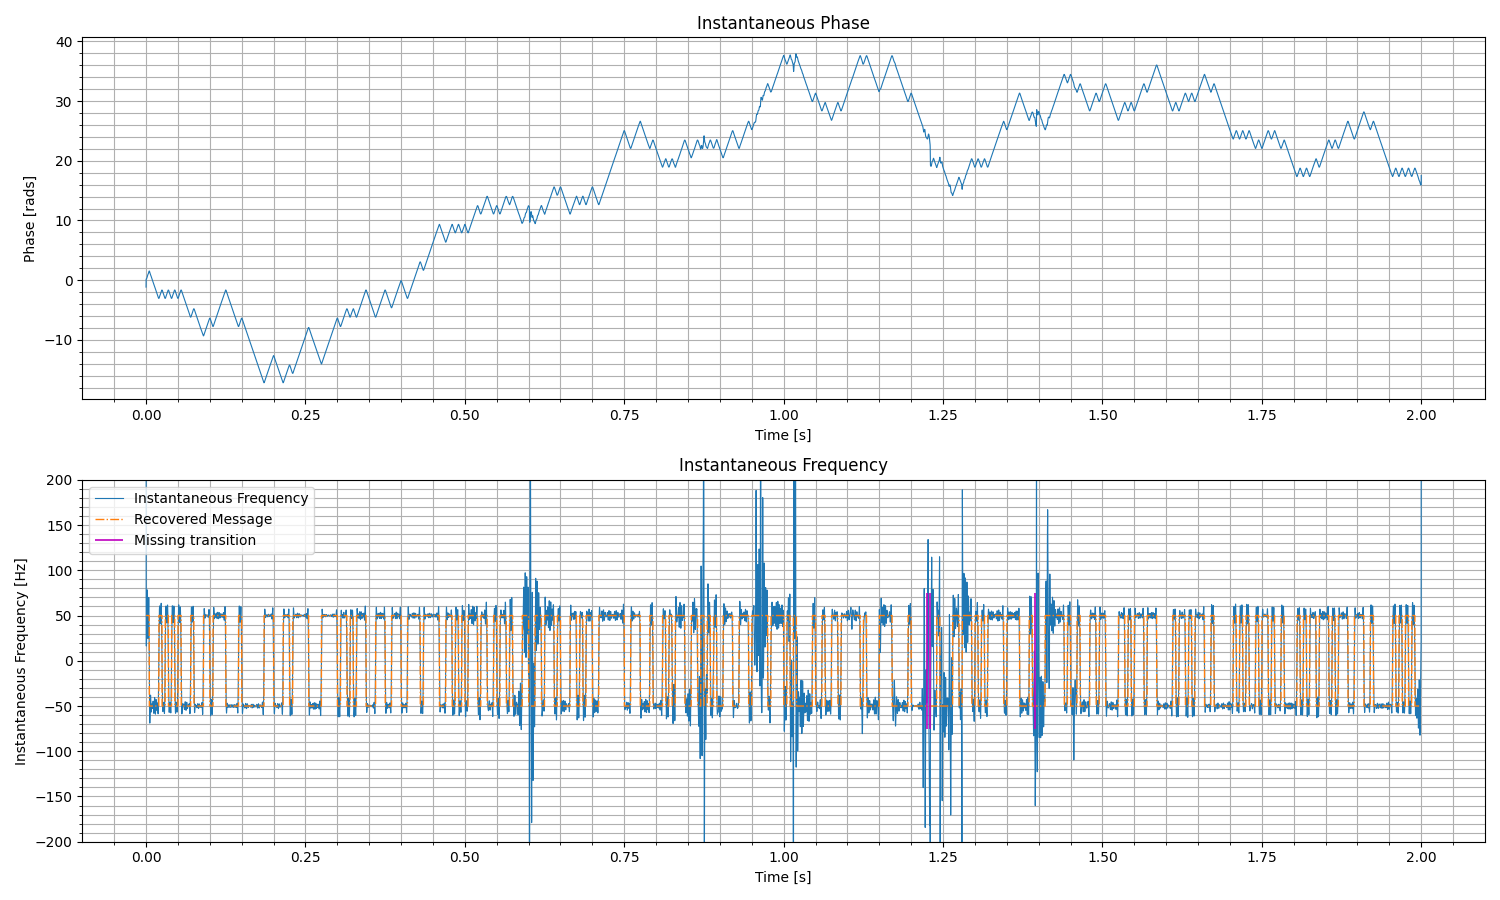
\includegraphics[width = \textwidth]{figs/sim/symRecovery/noiseFreq.png}
    \caption{Instantaneous Phase and Frequency of Noise Corrupted Ideal MSK signal.}
    \label{fig:noisefreq}
\end{figure}

\begin{figure}[h!]
    \centering
    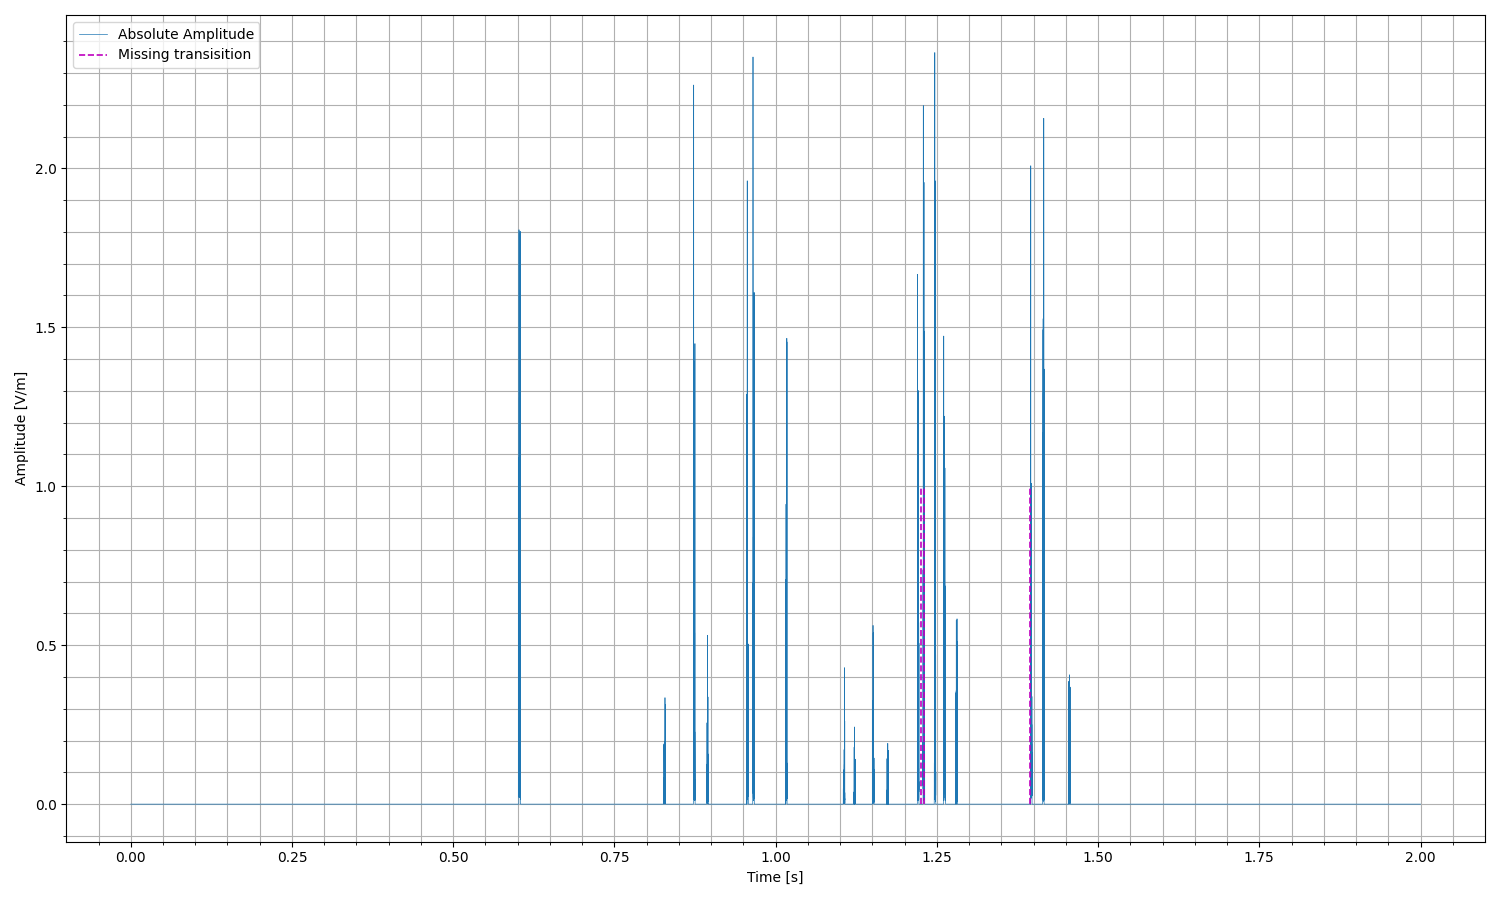
\includegraphics[width = \textwidth]{figs/sim/symRecovery/NoiseAmp.png}
    \caption{Absolute Amplitude of Simulated Noise Signal}
    \label{fig:noiseamp}
\end{figure}

\pagebreak
\subsection{Error Correction}
At this point further development is required in order to try and mitigate the bit loss. In order to do this it is important to further look at the signal characteristics. Although it is possible to estimate the BER and how many bits have been lost. The difficulty comes however in being able to locate where the missing bits have occured.


\subsubsection{Proximity}
One of the key features of MSK is that it is known exactly where the symbol changes will take place. The phasor will displace $\frac{\pi}{2}\si{\radian}$ for 1 symbol duration $T_b$. Hence a symbol change will happen only happen when displaces a multiple of $\frac{\pi}{2}$ from the last symbol change. In reality each change happens slightly less than $\frac{\pi}{2}$. As has previously been shown this results in 8 turning points in the complex plane. However the offset will be constant for each of these points relative to their respective axis, assuming zero initial phase. Using equation \ref{eq:offset} the relative closeness the axis can be shown, where $\phi_{bit}$ is the instantaneous phase at the point where there is a symbol change. The result of this calculation is shown by the figure \ref{fig:phaseHist}. This shows the distribution of the results of this calculation for a simulation run. As it is clear by the grouping of the ideal signal, this is where the transistions should occur. In the noise corrupted signal it is clear that that algorithm is using transitions that are not occurring in the correct place for a transition. In this example the BER corresponds to 7 missing bits. The bottom plot corresponds to the values specifically for the phase value where a bit error has occurred. For this example 4 of the errors have a value that categorises them with genuine transitions. This leaves only 3 bits that can be easily distinguished from the ideal signal. Using this information this clearly suggests that a suitable threshold might be created in order to help further narrow down the detected crossings that are suitable to be used as transition points, in order to prevent bit error.
\\\\
This metric although allows for further discrimination, it relies some form of phase syncronisation begin achieved, although no necessarily zero the initial phase needs to be a multiple of $\frac{\pi}{2}$ in order to extract suitable values, for thresholding. 
\begin{equation}
    \text{Offset} = \frac{\phi_{bit}}{\pi} \% \frac{1}{2}
    \label{eq:offset}
\end{equation}

\begin{figure}[h!]
    \centering
    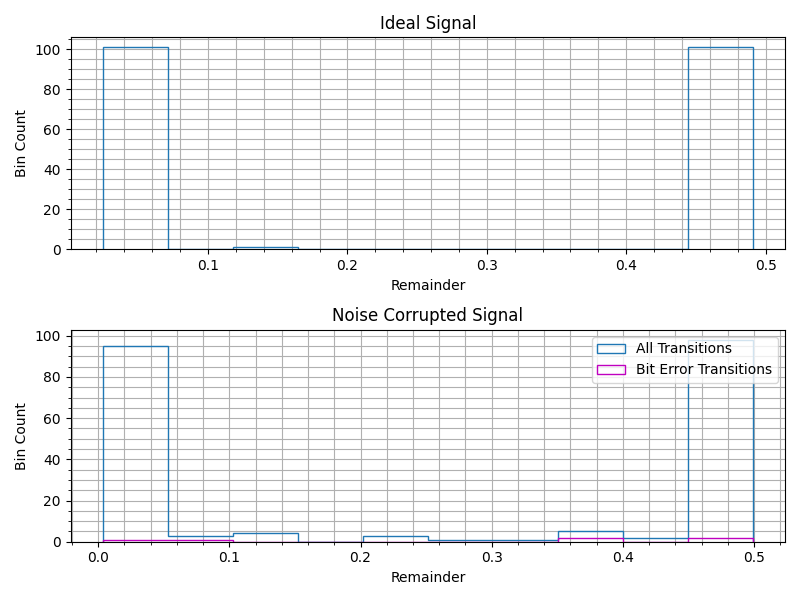
\includegraphics[width = \textwidth]{figs/error/phaseHist.png}
    \caption{\centering Histogram showing the results of $\frac{\phi_{bit}}{\pi} \%\left(\frac{1}{2}\right)$. \\ Top: Ideal signal with BER = -inf. \\ Bottom: Noise Corrupted Signal with BER = $e^{-4.20}$}
    \label{fig:phaseHist}
\end{figure}

\pagebreak
\subsubsection{Median Methods}
Figure \ref{fig:medgrad} shows the relationship between error and the median gradient of the phase between two points. As previously established for an MSK transmission the gradient should be equal to $\pm\frac{BW}{4}[Hz]$, in reality this value will be slightly less because of the shallower gradient surrounding the turning points. Despite this however for the ideal signal there clear groupings of the frequency values for the gradients in between each symbol transition. For the noise corrupted signal there is a much more variation away from these point with errors occurring at points where the median instantaneous frequency falls outside of these trends. Again as previously mentioned although the from this data a consistent cause of error is not obvious.

\begin{figure}[h!]
    \centering
    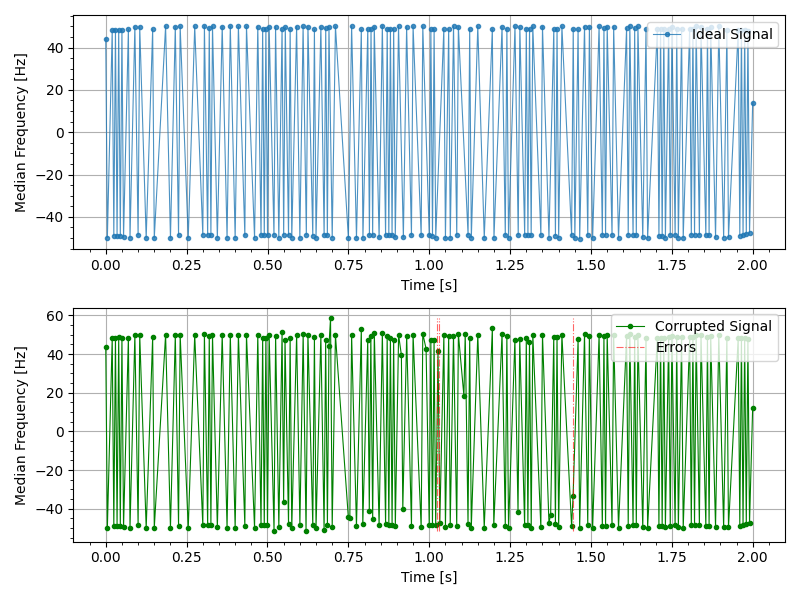
\includegraphics[width = \textwidth]{figs/error/medianGrad.png}
    \caption{\centering Median Gradient Values \\ Top: Ideal MSK \\ Bottom: Noise Corrupted MSK}
    \label{fig:medgrad}
\end{figure}

